% !TeX program = xelatex
% !BIB program = biber
\documentclass[light]{lutbeamer}
\usepackage{pgfpages}
\usepackage{ragged2e}
\usepackage{booktabs}
\usepackage{amssymb}
\usepackage{fontawesome5}
\usepackage{tikz}
\usepackage{pgfplots}
\pgfplotsset{compat=1.18}
\addbibresource{references.bib}

% ===================================================================
% METADATA (DERS KIMLIK BILGILERI)
% ===================================================================
\setdepartment{OSTIM Teknik Üniversitesi}
\institute{}
\author[Mühendislik Fakültesi]{\\
Prof.~Dr.~Yalçın ATA \\
Prof.~Dr.~Arif DEMİR \\
Dr.~Öğr.~Üyesi~Muhammed ELMNEFİ \\
Dr.~Öğr.~Üyesi~Haydar KILIÇ \\
Dr.~Öğr.~Üyesi~Emel GÜVEN \\
Dr.~Öğr.~Üyesi~Ufuk ASIL \\
Öğr.~Gör.~Sema ÇİFTÇİ
}
\title{MATH 204 -- Olasılık ve İstatistik}
\subtitle{Hafta 6: Sürekli Olasılık Dağılımları}
\date{2025--2026 Bahar Dönemi}

% ===================================================================
% SEMANTIK BOX VE RENK YARDIMCILARI
% ===================================================================
\definecolor{probExampleGreen}{HTML}{2E7D32}
\definecolor{probInfoGray}{HTML}{4B5563}
\definecolor{probSolutionBurgundy}{HTML}{7A1F2B}
\definecolor{probResultOrange}{HTML}{FF8621}

\setbeamercolor{block title example}{fg=white,bg=probExampleGreen}
\setbeamercolor{block body example}{fg=black,bg=probExampleGreen!10}

\newenvironment{infoblock}[1]
{
    \setbeamercolor{block title}{fg=white,bg=probInfoGray}
    \setbeamercolor{block body}{fg=black,bg=probInfoGray!10}
    \begin{block}{#1}
}
{
    \end{block}
}

\newenvironment{solutionblock}[1]
{
    \setbeamercolor{block title}{fg=white,bg=probSolutionBurgundy}
    \setbeamercolor{block body}{fg=black,bg=probSolutionBurgundy!8}
    \begin{beamercolorbox}[wd=\linewidth,sep=0.45ex,rounded=true]{block title}
        \usebeamerfont{block title}#1
    \end{beamercolorbox}
    \vspace{-0.25ex}
    \begin{beamercolorbox}[wd=\linewidth,sep=0.55ex,rounded=true,vmode]{block body}
    \footnotesize
    \setlength{\abovedisplayskip}{3pt}
    \setlength{\belowdisplayskip}{3pt}
    \setlength{\abovedisplayshortskip}{2pt}
    \setlength{\belowdisplayshortskip}{2pt}
    \setlength{\itemsep}{0.2em}
}
{
    \end{beamercolorbox}
}

\newenvironment{resultblock}[1]
{
    \setbeamercolor{block title}{fg=white,bg=probResultOrange}
    \setbeamercolor{block body}{fg=black,bg=probResultOrange!12}
    \begin{beamercolorbox}[wd=\linewidth,sep=0.40ex,rounded=true]{block title}
        \usebeamerfont{block title}#1
    \end{beamercolorbox}
    \vspace{-0.25ex}
    \begin{beamercolorbox}[wd=\linewidth,sep=0.50ex,rounded=true,vmode]{block body}
    \footnotesize
    \setlength{\abovedisplayskip}{2pt}
    \setlength{\belowdisplayskip}{2pt}
    \setlength{\abovedisplayshortskip}{1pt}
    \setlength{\belowdisplayshortskip}{1pt}
}
{
    \end{beamercolorbox}
}

\newenvironment{questionworkspace}
{
    \gdef\questionvisualcontent{
        \centering
        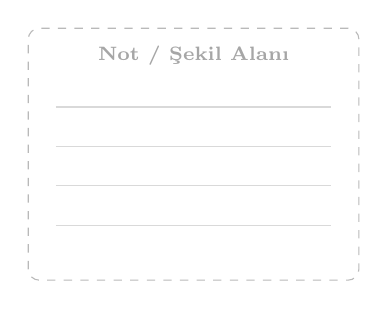
\begin{tikzpicture}[x=1cm,y=1cm]
            \draw[rounded corners, dashed, draw=gray!55] (0,0) rectangle (4.2,3.2);
            \node[font=\scriptsize\bfseries, text=gray!70] at (2.1,2.85) {Not / Şekil Alanı};
            \draw[gray!30] (0.35,2.2) -- (3.85,2.2);
            \draw[gray!30] (0.35,1.7) -- (3.85,1.7);
            \draw[gray!30] (0.35,1.2) -- (3.85,1.2);
            \draw[gray!30] (0.35,0.7) -- (3.85,0.7);
        \end{tikzpicture}
    }
    \begin{columns}[T,onlytextwidth]
        \begin{column}{0.48\textwidth}
            \begin{exampleblock}{Soru}
            \setlength{\abovedisplayskip}{3pt}
            \setlength{\belowdisplayskip}{3pt}
            \setlength{\abovedisplayshortskip}{2pt}
            \setlength{\belowdisplayshortskip}{2pt}
            \setlength{\itemsep}{0.2em}
}
{
            \end{exampleblock}
        \end{column}
        \begin{column}{0.48\textwidth}
            \questionvisualcontent
        \end{column}
    \end{columns}
}

\newcommand{\setquestionvisual}[1]{\gdef\questionvisualcontent{#1}}

\tikzset{
    qbox/.style={draw=black!65, rounded corners, fill=gray!6, minimum width=1.25cm, minimum height=0.55cm, align=center, font=\scriptsize},
    qgreen/.style={draw=probExampleGreen!75!black, rounded corners, fill=probExampleGreen!10, minimum width=1.25cm, minimum height=0.55cm, align=center, font=\scriptsize},
    qburg/.style={draw=probSolutionBurgundy!75!black, rounded corners, fill=probSolutionBurgundy!10, minimum width=1.25cm, minimum height=0.55cm, align=center, font=\scriptsize},
    qblue/.style={draw=blue!70!black, rounded corners, fill=blue!8, minimum width=1.25cm, minimum height=0.55cm, align=center, font=\scriptsize},
    qline/.style={-{Stealth[length=2.2mm]}, thick}
}

% ===================================================================
% AUTOMATIC TABLE OF CONTENTS (PRESENTATION FLOW)
% ===================================================================
\setcounter{tocdepth}{2}

\AtBeginSection[]{
  \begin{frame}{Sunum Planı}
    \scriptsize
    \begin{columns}[T]
      \begin{column}{0.48\textwidth}
        \tableofcontents[sections={1-4}, currentsection]
      \end{column}
      \begin{column}{0.48\textwidth}
        \tableofcontents[sections={5-10}, currentsection]
      \end{column}
    \end{columns}
  \end{frame}
}

\begin{document}

\setbeamertemplate{navigation symbols}{}
\setbeamertemplate{footline}{
  \begin{beamercolorbox}[wd=\paperwidth, ht=10pt, dp=1pt]{footline}
    \usebeamerfont{footline}
    \begin{tikzpicture}[remember picture,overlay]
      \node[anchor=south west, xshift=10mm, yshift=.4mm]
      at (current page.south west)
      {\insertshortauthor,~\department};
    \end{tikzpicture}
    \begin{tikzpicture}[remember picture,overlay]
      \node[anchor=south east, xshift=-5mm, yshift=0.5mm]
      at (current page.south east)
      {\insertframenumber \,/\, \inserttotalframenumber};
    \end{tikzpicture}
  \end{beamercolorbox}
}

% ===================================================================
% KAPAK SLAYTLARI
% ===================================================================

% Gorsel Tam Kapak (Logosuz)
\begin{frame}<article:0>[plain,noframenumbering]
  \begin{tikzpicture}[remember picture,overlay]
    \node[anchor=center, at=(current page.center), inner sep=0pt] {
      \includegraphics[width=\paperwidth, height=\paperheight]{logos/background_figure.jpg}
    };
  \end{tikzpicture}
\end{frame}

% Resmi Baslik Sayfasi (kapak icin ozel alt bilgi)
{
  \setbeamertemplate{footline}{
    \begin{beamercolorbox}[wd=\paperwidth, ht=10pt, dp=1pt]{footline}
      \usebeamerfont{footline}
      \begin{tikzpicture}[remember picture,overlay]
        \node[anchor=south west, xshift=10mm, yshift=.4mm, align=left]
        at (current page.south west)
        {\tiny Bu şablon OTU Yazılım Mühendisliği tarafından hazırlanmış olup \href{https://github.com/ufukasia/Ostim-Teknik--niversitesi-Yaz-l-m-M-hendisli-i---Lutbeamer-egitim-i-eri-i-haz-rlama-}{buradan} güncel haline ulaşabilirsiniz.};
      \end{tikzpicture}
      \begin{tikzpicture}[remember picture,overlay]
        \node[anchor=south east, xshift=-5mm, yshift=0.5mm]
        at (current page.south east)
        {\insertframenumber \,/\, \inserttotalframenumber};
      \end{tikzpicture}
    \end{beamercolorbox}
  }
  \maketitle{}
}

% GENEL ICERIK HARITASI
\begin{frame}{İçindekiler}
  \scriptsize
  \begin{columns}[T]
    \begin{column}{0.48\textwidth}
      \tableofcontents[sections={1-4}]
    \end{column}
    \begin{column}{0.48\textwidth}
      \tableofcontents[sections={5-10}]
    \end{column}
  \end{columns}
\end{frame}

\begin{frame}{Hafta 2--5'ten Ne Getiriyoruz?}
\small
\begin{columns}[T,onlytextwidth]
    \begin{column}{0.48\textwidth}
        \begin{infoblock}{Tekrarın Amacı}
            Bu bölüm, sürekli dağılımlara geçmeden önce olay olasılıkları ile dağılım düşüncesi arasındaki köprüyü yeniden kurar.
        \end{infoblock}

        \begin{itemize}
            \item Koşullu olasılık ve Bayes, bilgi güncellemenin dilidir.
            \item Rastgele değişken, olayları sayısal modele taşır.
            \item PMF, CDF, beklenen değer ve varyans; dağılımı okumak için temel araçlardır.
        \end{itemize}
    \end{column}
    \begin{column}{0.48\textwidth}
        \begin{resultblock}{Bu Haftaya Bağlantı}
            Sürekli dağılımlarda da aynı soruları soracağız:
            hangi değerler mümkün, hangi aralıklar daha olası, ortalama nerede ve yayılım ne kadar büyük?
        \end{resultblock}
    \end{column}
\end{columns}
\end{frame}

\begin{frame}{Bu Sunumu Nasıl Okumalıyız?}
\small
\begin{columns}[T,onlytextwidth]
    \begin{column}{0.48\textwidth}
        \begin{exampleblock}{Soru Frame'leri}
            Her soru artık tek başına bir bağlam anlatır. Sorunun bulunduğu frame'de çözüm yoktur; önce model kurmanız beklenir.
        \end{exampleblock}
    \end{column}
    \begin{column}{0.48\textwidth}
        \begin{solutionblock}{Çözüm Frame'leri}
            Çözümler bir alt frame'de, adım adım ilerler:
            modeli kur, doğru formülü seç, hesabı yap, sonucu yorumla.
        \end{solutionblock}
    \end{column}
\end{columns}
\end{frame}

% ===================================================================
% GENEL TEKRAR: MILESTONE TANIMLARI (Hafta 2--5)
% ===================================================================

\section{Genel Tekrar ve Sürekli Dağılımlara Köprü}
\subsection{Hafta 2--5'ten Ne Getiriyoruz?}

% ------------------------------------------------------------------
% MILESTONE 1: KOŞULLU OLASILIK
% ------------------------------------------------------------------
\begin{frame}{Tekrar 1: Koşullu Olasılık}
    \begin{columns}[T]
        \begin{column}{0.55\textwidth}
            \begin{block}{Tanım}
                $P(B)>0$ olmak koşuluyla, $B$ olayının gerçekleştiği bilindiğinde $A$ olayının olasılığı:
                \[
                P(A|B) = \frac{P(A \cap B)}{P(B)}
                \]
            \end{block}

            \begin{itemize}
                \item \textbf{Pay:} Her iki olayın da birlikte gerçekleşmesi.
                \item \textbf{Payda:} Koşulun olasılığı -- yeni evrenimiz.
                \item Koşullu olasılık da $0 \le P(A|B) \le 1$ aralığındadır.
            \end{itemize}
        \end{column}
        \begin{column}{0.42\textwidth}
            \begin{infoblock}{Sezgisel Yorum}
                Yeni bilgi geldiğinde örnek uzayımız \textbf{daralır}. Artık $S$ değil, $B$ kümesi yeni evrenimizdir.

                \vspace{0.2cm}
                $A \cap B$ kısımını, $B$'nin içindeki oranına göre normalize ederiz.
            \end{infoblock}
        \end{column}
    \end{columns}
\end{frame}

\begin{frame}[t]{Soru 1: Termal Testten Sonra Titreşim Başarısı}
\small
\begin{questionworkspace}
    Bir pil modülü üretim hattında gün sonunda raporlanan 150 modülün tamamı \textbf{termal testi geçmiştir} ($Te$). Aynı grup içinden 120 modülün \textbf{titreşim testini de geçtiği} ($Ti$) görülmüştür.

    \vspace{0.15cm}
    Termal testi geçtiği \textbf{zaten bilinen} bir modül seçildiğinde, bu modülün titreşim testini de geçmiş olma olasılığı nedir? Yani $P(Ti \mid Te)$ değerini bulunuz.
    \setquestionvisual{
        \centering
        \begin{tikzpicture}[scale=0.85, every node/.style={font=\scriptsize}]
            \node[qblue, minimum width=3.2cm, minimum height=0.9cm] (t) at (2.1,3.0) {Termal testi \\ geçen 150 modül};
            \node[qgreen, minimum width=2.6cm, minimum height=0.9cm] (v) at (2.1,1.2) {Titreşimi de \\ geçen 120};
            \draw[qline] (t) -- (v);
            \node at (2.1,2.1) {koşul: $Te$};
        \end{tikzpicture}
    }
\end{questionworkspace}
\end{frame}

\begin{frame}[shrink=8]{Soru 1: Termal Testten Sonra Titreşim Başarısı Çözümü}
\small
\begin{solutionblock}{Adım 1: Koşullu olasılığı doğru olaya bağla}
    İstenen olay, \textbf{termal testi geçtiği bilinen} bir modül için titreşim başarısıdır. Bu nedenle
    \[
    P(Ti \mid Te)=\frac{P(Ti \cap Te)}{P(Te)}
    \]
    formülünü kullanırız.
\end{solutionblock}

\begin{solutionblock}{Adım 2: Sayımları koşullu olasılık oranına yerleştir}
    Veri doğrudan sayım verdiği için paya iki testi de geçen modül sayısını, paydaya termal testi geçen modül sayısını koyarız:
    \[
    P(Ti \mid Te)=\frac{120}{150}=0.80
    \]
\end{solutionblock}

\begin{resultblock}{Yorum}
    Termal testi geçen modüllerin yaklaşık \%80'i titreşim testini de geçmektedir. Yani ikinci testte hâlâ anlamlı bir eleme vardır; iki test aynı bilgiyi vermemektedir.
\end{resultblock}
\end{frame}

% ------------------------------------------------------------------
% MILESTONE 2: ÇARPIM KURALI
% ------------------------------------------------------------------
\begin{frame}[fragile]
    \frametitle{Tekrar 2: Çarpım Kuralı}
    \begin{block}{İki Olay İçin}
        Koşullu olasılık tanımından:
        \[
        P(A \cap B) = P(B) \cdot P(A|B) = P(A) \cdot P(B|A)
        \]
    \end{block}

    \begin{block}{Zincir Kuralı ($k$ Olay)}
        \[
        P(A_1 \cap A_2 \cap \cdots \cap A_k)
        = P(A_1)\, P(A_2|A_1)\, P(A_3|A_1 \cap A_2) \cdots
        \]
    \end{block}

    \begin{infoblock}{Uygulama Alanı}
        Yerine koymadan çekim problemlerinde (kart, sigorta, top çekme) her adımda havuz küçülür; koşullu olasılıklar buna göre güncellenir.
    \end{infoblock}
\end{frame}

\begin{frame}[t]{Soru 2: İki Testi Birden Geçen Kontrol Kartı}
\small
\begin{questionworkspace}
    Bir kontrol kartı önce \textbf{optik incelemeyi geçiyor} ($Op$), ardından \textbf{fonksiyonel testi geçiyor} ($Fn$). Bu kart için $P(Op)=0.93$ ve $P(Fn \mid Op)=0.96$ veriliyor.

    \vspace{0.15cm}
    Rastgele seçilen bir kartın \textbf{iki testi de} geçme olasılığı nedir? Yani $P(Op \cap Fn)$ değerini bulunuz.
    \setquestionvisual{
        \centering
        \begin{tikzpicture}[scale=0.95, every node/.style={font=\scriptsize}]
            \node[qblue, minimum width=1.2cm] (kart) at (0, 0.6) {Kart};
            \node[qgreen, minimum width=1.2cm] (op) at (2.4, 0.6) {$Op$ (Optik)};
            \node[qgreen, minimum width=1.2cm] (fn) at (5.1, 0.6) {$Fn$ (Fonks.)};
            
            \draw[qline] (kart) -- node[above] {$P(Op)$} node[below] {$0.93$} (op);
            \draw[qline] (op) -- node[above] {$P(Fn \mid Op)$} node[below] {$0.96$} (fn);
            
            \draw[qline, dashed, draw=probSolutionBurgundy] 
                 (kart.south) to[bend right=35] 
                 node[below, text=probSolutionBurgundy] {$P(Op \cap Fn) = \text{?}$} (fn.south);
        \end{tikzpicture}
    }
\end{questionworkspace}
\end{frame}

\begin{frame}[shrink=8]{Soru 2: İki Testi Birden Geçen Kontrol Kartı Çözümü}
\small
\begin{solutionblock}{Adım 1: Olay sırasını kur}
    Önce optik inceleme, sonra fonksiyonel test vardır. Bu yüzden kesişim olasılığı çarpım kuralıyla yazılır:
    \[
    P(Op \cap Fn)=P(Op)\,P(Fn \mid Op)
    \]
\end{solutionblock}

\begin{solutionblock}{Adım 2: Sayısal değeri hesapla}
    \[
    P(Op \cap Fn)=0.93 \times 0.96 = 0.8928
    \]
    Yani her iki testi de geçen kartların oranı 0.8928'dir.
\end{solutionblock}

\begin{resultblock}{Yorum}
    Süreç iki aşamalı olduğu için toplam başarı oranı tek tek başarı oranlarından küçüktür. Yaklaşık \%89.28'lik oran, ikinci testin de eleme yaptığını gösterir.
\end{resultblock}
\end{frame}

% ------------------------------------------------------------------
% MILESTONE 3: BAĞIMSIZLIK
% ------------------------------------------------------------------
\begin{frame}{Tekrar 3: Bağımsızlık}
    \begin{columns}[T]
        \begin{column}{0.48\textwidth}
            \begin{block}{Tanım}
                İki olay $A$ ve $B$ \textbf{bağımsızdır} $\iff$
                \[
                P(A \cap B) = P(A)\, P(B)
                \]
                Eşdeğer ifade: $P(A|B) = P(A)$.
            \end{block}

            \begin{itemize}
                \item $B$'yi bilmek, $A$'nın olasılığını \textbf{değiştirmez}.
                \item $A$ ve $B$ bağımsızsa $\Rightarrow$ $A'$ ve $B$ de bağımsızdır.
            \end{itemize}
        \end{column}
        \begin{column}{0.48\textwidth}
            \begin{alertblock}{Dikkat: Ayrıklık $\neq$ Bağımsızlık}
                \textbf{Ayrık:} $A \cap B = \emptyset$ $\Rightarrow$ $P(A \cap B)=0$.

                \vspace{0.15cm}
                İki pozitif olasılıklı olay hem ayrık hem bağımsız \textbf{olamaz}; çünkü $P(A)P(B) > 0 \neq 0$.
            \end{alertblock}
        \end{column}
    \end{columns}
\end{frame}

\begin{frame}[t]{Soru 3: İki Yedek Güç Ünitesinin Birlikte Hazır Olması}
\small
\begin{questionworkspace}
    Bir veri merkezinde birbirinden bağımsız çalışan iki yedek güç ünitesi vardır. \textbf{1. ünitenin hazır olması} olayını $Hz_1$, \textbf{2. ünitenin hazır olması} olayını $Hz_2$ ile gösterelim. Veriler $P(Hz_1)=0.98$ ve $P(Hz_2)=0.95$ şeklindedir.

    \vspace{0.15cm}
    İki ünitenin aynı anda çalışır durumda olma olasılığı nedir? Yani $P(Hz_1 \cap Hz_2)$ değerini bulunuz.
    \setquestionvisual{
        \centering
        \begin{tikzpicture}[scale=0.78, every node/.style={font=\scriptsize}]
            \node[qgreen, minimum width=1.6cm] (u1) at (1.1,2.0) {Ünite 1\\$0.98$};
            \node[qgreen, minimum width=1.6cm] (u2) at (3.4,2.0) {Ünite 2\\$0.95$};
            \node[qbox, minimum width=2.0cm] (and) at (2.25,0.7) {Birlikte\\hazır};
            \draw[qline] (u1) -- (and);
            \draw[qline] (u2) -- (and);
        \end{tikzpicture}
    }
\end{questionworkspace}
\end{frame}

\begin{frame}[shrink=8]{Soru 3: İki Yedek Güç Ünitesinin Birlikte Hazır Olması Çözümü}
\small
\begin{solutionblock}{Adım 1: Bağımsızlık bilgisini kullan}
    Olaylar bağımsız olduğundan kesişim olasılığı doğrudan çarpım olarak yazılır:
    \[
    P(Hz_1 \cap Hz_2)=P(Hz_1)\,P(Hz_2)
    \]
\end{solutionblock}

\begin{solutionblock}{Adım 2: Çarpımı hesapla}
    \[
    P(Hz_1 \cap Hz_2)=0.98 \times 0.95 = 0.931
    \]
\end{solutionblock}

\begin{resultblock}{Yorum}
    İki ünitenin birlikte hazır olma olasılığı yaklaşık \%93.1'dir. Bağımsızlık varsayımı olmasaydı bu çarpımı doğrudan yapamazdık.
\end{resultblock}
\end{frame}

\begin{frame}[shrink=6,t]{Soru 4: Seri-Paralel Karma Sistemin Güvenilirliği}
\scriptsize
\begin{questionworkspace}
    Aşağıdaki elektrik devresinde 1. bileşen, ortadaki paralel blok ve 4. bileşen \textbf{seri}; orta bloktaki 2. ve 3. bileşenler ise \textbf{paralel} bağlıdır.

    \vspace{0.15cm}
    $i$. bileşenin $t$ zamanından önce arızalanma olayını $Ar_i$ ile gösterelim. Veriler
    \[
    \begin{aligned}
    P(Ar_1)&=0.10,\quad P(Ar_2)=0.20,\\
    P(Ar_3)&=0.25,\quad P(Ar_4)=0.15
    \end{aligned}
    \]
    olup bileşen ömürlerinin bağımsız olduğu kabul ediliyor.

    \vspace{0.15cm}
    Sistemin $t$ zamanından önce arızalanma olasılığı nedir? Yani $P(Ar_{\text{sistem}})$ değerini bulunuz.
    \setquestionvisual{
        \centering
        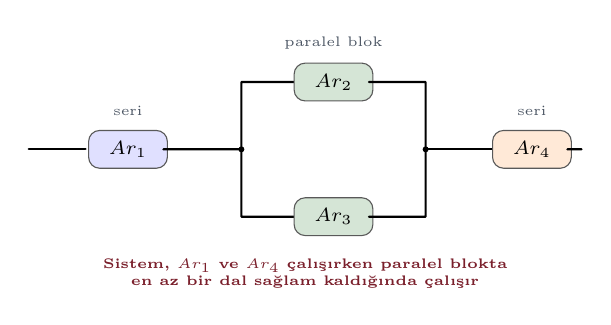
\begin{tikzpicture}[scale=0.9, every node/.style={font=\scriptsize}, line cap=round, line join=round]
            \coordinate (in) at (0.0,1.5);
            \coordinate (a) at (0.8,1.5);
            \coordinate (b) at (2.0,1.5);
            \coordinate (split) at (3.0,1.5);
            \coordinate (merge) at (5.6,1.5);
            \coordinate (c) at (6.6,1.5);
            \coordinate (out) at (7.8,1.5);

            \draw[thick] (in) -- (a);
            \node[qbox, minimum width=1.0cm, minimum height=0.48cm, fill=blue!12] at (1.4,1.5) {$Ar_1$};
            \draw[thick] (1.9,1.5) -- (split);

            \draw[thick] (split) -- (3.0,2.45) -- (3.8,2.45);
            \draw[thick] (split) -- (3.0,0.55) -- (3.8,0.55);
            \node[qbox, minimum width=1.0cm, minimum height=0.48cm, fill=probExampleGreen!20] at (4.3,2.45) {$Ar_2$};
            \node[qbox, minimum width=1.0cm, minimum height=0.48cm, fill=probExampleGreen!20] at (4.3,0.55) {$Ar_3$};
            \draw[thick] (4.8,2.45) -- (5.6,2.45) -- (merge);
            \draw[thick] (4.8,0.55) -- (5.6,0.55) -- (merge);

            \draw[thick] (merge) -- (c);
            \node[qbox, minimum width=1.0cm, minimum height=0.48cm, fill=probResultOrange!18] at (7.1,1.5) {$Ar_4$};
            \draw[thick] (7.6,1.5) -- (out);

            \fill (split) circle (1.2pt);
            \fill (merge) circle (1.2pt);
            \node[font=\tiny, text=probInfoGray] at (1.4,2.05) {seri};
            \node[font=\tiny, text=probInfoGray] at (4.3,3.0) {paralel blok};
            \node[font=\tiny, text=probInfoGray] at (7.1,2.05) {seri};
            \node[font=\tiny\bfseries, text=probSolutionBurgundy, text width=5.4cm, align=center] at (3.9,-0.25) {Sistem, $Ar_1$ ve $Ar_4$ çalışırken paralel blokta en az bir dal sağlam kaldığında çalışır};
        \end{tikzpicture}
    }
\end{questionworkspace}
\end{frame}

\begin{frame}[shrink=8]{Soru 4: Seri-Paralel Karma Sistemin Güvenilirliği Çözümü}
\scriptsize
\begin{solutionblock}{Adım 1: Önce sistemin çalışma olayını kur}
    Hesabı doğrudan arıza üzerinden yapmak yerine tümleyenden gitmek daha temizdir. $Ca_i=Ar_i'$ ile ``$i$. bileşen çalışır'' olayını gösterelim. O zaman
    \[
    P(Ca_1)=0.90,\quad P(Ca_2)=0.80,\quad P(Ca_3)=0.75,\quad P(Ca_4)=0.85
    \]
    olur.
\end{solutionblock}

\begin{solutionblock}{Adım 2: Paralel bloğun çalışma olasılığını bul}
    Orta blokta 2. ve 3. bileşenler paraleldir. Bu blok ancak \textbf{ikisi birden arızalanırsa} durur:
    \[
    P(Ca_{23})=1-P(Ar_2 \cap Ar_3)=1-(0.20)(0.25)=1-0.05=0.95
    \]
\end{solutionblock}

\begin{solutionblock}{Adım 3: Seri yapıyı kullanarak sistemin çalışma olasılığını hesapla}
    Tüm sistemin çalışması için 1. bileşen, paralel blok ve 4. bileşen birlikte çalışmalıdır:
    \[
    P(Ca_{\text{sistem}})=P(Ca_1)\,P(Ca_{23})\,P(Ca_4)
    =0.90 \times 0.95 \times 0.85=0.72675
    \]
\end{solutionblock}

\begin{solutionblock}{Adım 4: Tümleyenden sistem arızasını bul}
    \[
    P(Ar_{\text{sistem}})=1-P(Ca_{\text{sistem}})
    =1-0.72675=0.27325
    \]
\end{solutionblock}

\begin{resultblock}{Yorum}
    Sonuç olarak sistemin $t$ zamanından önce arızalanma olasılığı \%27.325'tir. Paralel blok orta kısmı güçlendirir; ancak iki seri bileşen olduğu için sistem hâlâ bu bileşenlerin zayıflığına duyarlıdır.
\end{resultblock}
\end{frame}

% ------------------------------------------------------------------
% MILESTONE 4: TOPLAM OLASILIK TEOREMİ
% ------------------------------------------------------------------
\begin{frame}[fragile]
    \frametitle{Tekrar 4: Toplam Olasılık Teoremi}
    \begin{columns}[T]
        \begin{column}{0.55\textwidth}
            \begin{block}{Teorem}
                $B_1, B_2, \dots, B_k$ örneklem uzayının bir bölüntüsü ise:
                \[
                P(A) = \sum_{i=1}^{k} P(B_i)\, P(A|B_i)
                \]
            \end{block}

            \begin{itemize}
                \item Her terim bir ``dal olasılığı'': Kaynağın ağırlığı $\times$ o kaynaktan $A$ çıkma oranı.
                \item Tüm dalların toplamı $A$'nın genel olasılığını verir.
            \end{itemize}
        \end{column}
        \begin{column}{0.42\textwidth}
            \centering
            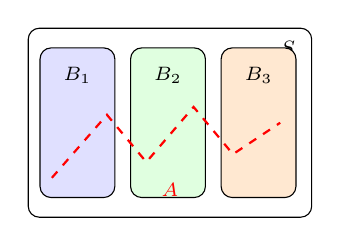
\begin{tikzpicture}[x=1cm,y=1cm,every node/.style={font=\scriptsize}]
                \draw[rounded corners] (0,0) rectangle (3.6,2.4);
                \node at (3.3,2.15) {$S$};
                \draw[fill=blue!12,rounded corners] (0.15,0.25) rectangle (1.1,2.15);
                \draw[fill=green!12,rounded corners] (1.3,0.25) rectangle (2.25,2.15);
                \draw[fill=orange!18,rounded corners] (2.45,0.25) rectangle (3.4,2.15);
                \node at (0.625,1.8) {$B_1$};
                \node at (1.775,1.8) {$B_2$};
                \node at (2.925,1.8) {$B_3$};
                \draw[thick, red, dashed] (0.3,0.5) -- (1.0,1.3) -- (1.5,0.7) -- (2.1,1.4) -- (2.6,0.8) -- (3.2,1.2);
                \node[red] at (1.8,0.35) {$A$};
            \end{tikzpicture}

            \vspace{0.2cm}
            \scriptsize $A$, farklı kaynaklardan ($B_i$) gelen parçaların birleşimidir.
        \end{column}
    \end{columns}
\end{frame}

\begin{frame}[shrink=8,t]{Soru 5: Üretim Hatlarından Gelen Hurda Olasılığı}
\small
\begin{questionworkspace}
    Bir fabrikada üç üretim hattı günlük toplam üretimin sırasıyla \%50, \%30 ve \%20'sini karşılıyor. Parçanın 1., 2. ve 3. hattan gelme olaylarını $Ht_1$, $Ht_2$, $Ht_3$; parçanın hurdalı çıkma olayını $Hu$ ile gösterelim. Hatlara göre hurda oranları
    \[
    \begin{aligned}
    P(Hu \mid Ht_1)&=0.02 \\
    P(Hu \mid Ht_2)&=0.03 \\
    P(Hu \mid Ht_3)&=0.05
    \end{aligned}
    \]
    olarak veriliyor.

    Günlük üretimden rastgele seçilen bir parçanın hurdalı olma olasılığı nedir? Yani $P(Hu)$ değerini bulunuz.
    \setquestionvisual{
        \centering
        \renewcommand{\arraystretch}{1.2}
        \setlength{\tabcolsep}{6pt}
        \begin{tabular}{@{}lcc@{}}
            \toprule
            Hat & Pay & $P(Hu \mid \cdot)$ \\ \midrule
            $Ht_1$ & 0.50 & 0.02 \\
            $Ht_2$ & 0.30 & 0.03 \\
            $Ht_3$ & 0.20 & 0.05 \\ \bottomrule
        \end{tabular}
    }
\end{questionworkspace}
\end{frame}

\begin{frame}[shrink=8]{Soru 5: Üretim Hatlarından Gelen Hurda Olasılığı Çözümü}
\small
\begin{solutionblock}{Adım 1: Toplam olasılık teoremini kur}
    Parçanın hurdalı olması, $Ht_1$, $Ht_2$ veya $Ht_3$ hattından gelmesine bağlıdır. Bu nedenle
    \[
    P(Hu)=P(Ht_1)P(Hu \mid Ht_1)+P(Ht_2)P(Hu \mid Ht_2)+P(Ht_3)P(Hu \mid Ht_3)
    \]
    yazılır.
\end{solutionblock}

\begin{solutionblock}{Adım 2: Hat payları ile hurda oranlarını çarp}
    \[
    P(Hu)=0.50(0.02)+0.30(0.03)+0.20(0.05)
    \]
    \[
    =0.010+0.009+0.010=0.029
    \]
\end{solutionblock}

\begin{resultblock}{Yorum}
    Günlük üretim içinden seçilen bir parçanın hurdalı çıkma olasılığı \%2.9'dur. Toplam olasılık, farklı kaynakların ağırlıklı katkısını tek sayıda toplar.
\end{resultblock}
\end{frame}

% ------------------------------------------------------------------
% MILESTONE 5: BAYES TEOREMİ
% ------------------------------------------------------------------
\begin{frame}[fragile]
    \frametitle{Tekrar 5: Bayes Teoremi}
    \begin{block}{Teorem}
        $B_1, \dots, B_k$ bir bölüntü ve $P(A) > 0$ olsun. Gözlem $A$ yapıldığında, bunun $r$'inci kaynaktan gelme olasılığı:
        \[
        P(B_r | A) = \frac{P(B_r)\, P(A|B_r)}{\displaystyle\sum_{i=1}^{k} P(B_i)\, P(A|B_i)}
        \]
    \end{block}

    \begin{columns}[T]
        \begin{column}{0.48\textwidth}
            \begin{infoblock}{Okuma Yöntemi}
                \begin{itemize}
                    \item \textbf{Pay:} $r$'inci dalın katkısı.
                    \item \textbf{Payda:} Toplam Olasılık ($P(A)$).
                    \item Sonuçtan sebebe giden yol.
                \end{itemize}
            \end{infoblock}
        \end{column}
        \begin{column}{0.48\textwidth}
            \begin{alertblock}{En Sık Yapılan Hata}
                \[
                P(A|B) \neq P(B|A)
                \]
                Bayes teoremi bu iki yönü birbirine dönüştürme aracıdır.
            \end{alertblock}
        \end{column}
    \end{columns}
\end{frame}

\begin{frame}[t]{Soru 6: Hurdalı Parçanın Kaynağını Geri Bulmak}
\small
\begin{questionworkspace}
    Bir önceki örnekteki üç üretim hattı için günlük toplam hurda olasılığı
    \[
    P(Hu)=0.029
    \]
    olarak bulunmuştu. Parçanın 3. hattan gelme olayını $Ht_3$, hurdalı olma olayını $Hu$ ile gösterirsek ayrıca
    \[
    P(Ht_3)=0.20,\qquad P(Hu \mid Ht_3)=0.05
    \]
    bilgileri veriliyor.

    \vspace{0.15cm}
    Hurdalı olduğu görülen bir parçanın 3. hattan gelmiş olma olasılığı nedir? Yani $P(Ht_3 \mid Hu)$ değerini bulunuz.
    \setquestionvisual{
        \centering
        \renewcommand{\arraystretch}{1.3}
        \setlength{\tabcolsep}{8pt}
        \begin{tabular}{@{}lcc@{}}
            \toprule
            Kaynak & Önsel & Hurda \\ \midrule
            $Ht_1$ & 0.50 & 0.02 \\
            $Ht_2$ & 0.30 & 0.03 \\
            \textcolor{probSolutionBurgundy}{$Ht_3$} & \textcolor{probSolutionBurgundy}{0.20} & \textcolor{probSolutionBurgundy}{0.05} \\ \bottomrule
        \end{tabular}

        \vspace{0.15cm}
        {\scriptsize Bayes: $Hu$ gözlemi sonrası $Ht_3$'ün payı büyür.}
    }
\end{questionworkspace}
\end{frame}

\begin{frame}[shrink=8]{Soru 6: Hurdalı Parçanın Kaynağını Geri Bulmak Çözümü}
\small
\begin{solutionblock}{Adım 1: Bayes teoremi ile ters koşullu olasılığı yaz}
    Elimizde $P(Hu \mid Ht_3)$ var; istenen ise $P(Ht_3 \mid Hu)$'dur. Bu dönüşüm için Bayes teoremi kullanılır:
    \[
    P(Ht_3 \mid Hu)=\frac{P(Ht_3)\,P(Hu \mid Ht_3)}{P(Hu)}
    \]
\end{solutionblock}

\begin{solutionblock}{Adım 2: Sayısal değerleri yerine koy}
    \[
    P(Ht_3 \mid Hu)=\frac{0.20 \times 0.05}{0.029}
    =\frac{0.010}{0.029}\approx 0.345
    \]
\end{solutionblock}

\begin{resultblock}{Yorum}
    Hurdalı bir parçanın 3. hattan gelmiş olma olasılığı yaklaşık \%34.5'tir. 3. hat toplam üretimin yalnızca \%20'sini yapmasına rağmen hurda oranı yüksek olduğu için, hurdalı parça içinde payı büyümüştür.
\end{resultblock}
\end{frame}

% ------------------------------------------------------------------
% MILESTONE 6: RASTGELE DEĞİŞKEN
% ------------------------------------------------------------------
\begin{frame}{Tekrar 6: Rastgele Değişken Kavramı}
    \begin{columns}[T]
        \begin{column}{0.55\textwidth}
            \begin{block}{Tanım}
                Rastgele değişken, örnek uzaydaki \textbf{her elemana bir reel sayı atayan} fonksiyondur:
                \[
                X : S \to \mathbb{R}, \qquad \omega \mapsto X(\omega).
                \]
            \end{block}

            \begin{itemize}
                \item $X$: Değişkenin adı (büyük harf).
                \item $x$: Aldığı belirli bir değer (küçük harf).
                \item Olayları sayılara çevirerek \textbf{istatistiğe köprü} kurar.
            \end{itemize}
        \end{column}
        \begin{column}{0.42\textwidth}
            \begin{infoblock}{İki Temel Tür}
                \begin{itemize}
                    \item \textbf{Ayrık:} Değer kümesi sayılabilir.

                    $X \in \{0,1,2,\dots\}$ (adet, sayım).
                    \item \textbf{Sürekli:} Değer kümesi bir aralık.

                    $X \in [a,b]$ (ölçüm, süre).
                \end{itemize}
            \end{infoblock}
        \end{column}
    \end{columns}
\end{frame}

\begin{frame}[t]{Soru 7: Hatalı Lehim Noktası Sayısı}
\small
\begin{questionworkspace}
    Bir baskı devre kartında 4 kritik lehim noktası tek tek kontrol ediliyor. Her nokta ya hatalı ya da hatasız olarak sınıflandırılıyor.

    \vspace{0.15cm}
    $X=$ ``kart üzerindeki hatalı lehim noktası sayısı'' olarak tanımlansın.

    \vspace{0.15cm}
    $X$ hangi değerleri alabilir ve bu değişkenin türü nedir?
    \setquestionvisual{
        \centering
        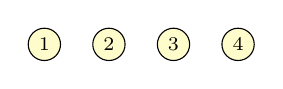
\begin{tikzpicture}[scale=0.82, every node/.style={font=\scriptsize}]
            \foreach \i/\x in {1/0.7,2/1.7,3/2.7,4/3.7}{
                \draw[fill=yellow!20] (\x,1.8) circle (0.25);
                \node at (\x,1.8) {\i};
            }
        \end{tikzpicture}
    }
\end{questionworkspace}
\end{frame}

\begin{frame}[shrink=8]{Soru 7: Hatalı Lehim Noktası Sayısı Çözümü}
\small
\begin{solutionblock}{Adım 1: Sayım değişkeninin olası değerlerini listele}
    Dört kontrol noktasının hiçbiri hatalı olmayabilir, yalnızca biri hatalı olabilir veya dört noktanın tamamı hatalı olabilir. Bu nedenle
    \[
    X \in \{0,1,2,3,4\}
    \]
    olur.
\end{solutionblock}

\begin{solutionblock}{Adım 2: Türünü belirle}
    Bu değer kümesi sonlu ve sayılabilirdir. Dolayısıyla $X$, \textbf{ayrık rastgele değişken}dir.
\end{solutionblock}

\begin{resultblock}{Yorum}
    Rastgele değişken tanımlamanın özü, fiziksel bir kalite kontrol olayını sayısal bir büyüklüğe dönüştürmektir. Bu dönüşüm daha sonra PMF, CDF ve beklenen değer hesaplarına kapı açar.
\end{resultblock}
\end{frame}

\begin{frame}[t]{Soru 8: Dört Denetimde Net Geçiş Dengesi}
\scriptsize
\begin{questionworkspace}
    Bir seri üretim hattında art arda 4 kalite denetimi yapılıyor. Her denetim ya \textbf{başarıyla geçiliyor} ya da \textbf{geçilemiyor}.

    \vspace{0.15cm}
    Başarıyla geçilen denetim sayısı $G$, geçilemeyen denetim sayısı $K$ olsun. Net denetim dengesini gösteren rastgele değişken
    \[
    W=G-K
    \]
    olarak tanımlanıyor.

    \vspace{0.15cm}
    $W$'nin alabileceği tüm olası değerleri listeleyiniz.
    \setquestionvisual{
        \centering
        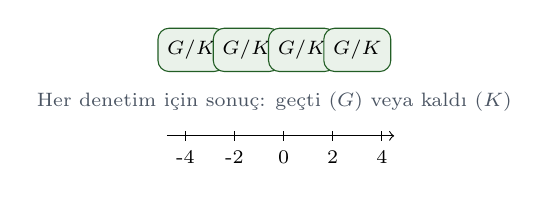
\begin{tikzpicture}[scale=0.78, every node/.style={font=\scriptsize}]
            \foreach \i/\x in {1/0.7,2/1.6,3/2.5,4/3.4}{
                \node[qgreen, minimum width=0.72cm] at (\x,2.2) {$G/K$};
            }
            \draw[->] (0.3,0.8) -- (4.0,0.8);
            \foreach \v/\x in {-4/0.6,-2/1.4,0/2.2,2/3.0,4/3.8}{
                \draw (\x,0.72) -- (\x,0.88);
                \node[below] at (\x,0.72) {\v};
            }
            \node[text=probInfoGray] at (2.05,1.35) {Her denetim için sonuç: geçti $(G)$ veya kaldı $(K)$};
        \end{tikzpicture}
    }
\end{questionworkspace}
\end{frame}

\begin{frame}{Soru 8: Dört Denetimde Net Geçiş Dengesi Çözümü}
\scriptsize
\begin{columns}[T,onlytextwidth]
    \begin{column}{0.48\textwidth}
        \begin{solutionblock}{Adım 1: Yardımcı ilişkiyi kur}
            Toplam 4 denetim olduğundan
            \[
            G+K=4
            \]
            olur. Buradan
            \[
            K=4-G
            \]
            yazılır.
        \end{solutionblock}
    \end{column}
    \begin{column}{0.48\textwidth}
        \begin{solutionblock}{Adım 2: $W$'yi tek değişken cinsinden yaz}
            \[
            W=G-K=G-(4-G)=2G-4
            \]
            Ayrıca $G$ yalnızca
            \[
            G=0,1,2,3,4
            \]
            değerlerini alabilir.
        \end{solutionblock}
    \end{column}
\end{columns}

\begin{resultblock}{Yorum}
    Buna göre
    \[
    G=0,1,2,3,4 \Longrightarrow W=-4,-2,0,2,4
    \]
    olur. Yani $W$ yalnızca $\{-4,-2,0,2,4\}$ değerlerini alır.
\end{resultblock}
\end{frame}

\begin{frame}[t]{Soru 9: Vale Teslimatında Doğru Anahtar Sayısı}
\scriptsize
\begin{questionworkspace}
    Bir vale, Alice, Bob ve Charlie'ye ait 3 anahtarı karıştırıyor ve anahtarları müşterilere rastgele geri veriyor.

    \vspace{0.15cm}
    Doğru anahtarı alan müşteri sayısını gösteren rastgele değişken $M$ olsun.

    \vspace{0.15cm}
    $M$'nin alabileceği olası değerler nelerdir?
    \setquestionvisual{
        \centering
        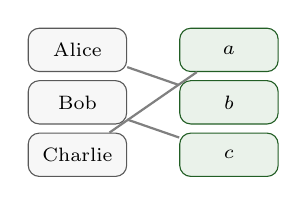
\begin{tikzpicture}[scale=0.74, every node/.style={font=\scriptsize}]
            \node[qbox] (a) at (0.7,2.3) {Alice};
            \node[qbox] (b) at (0.7,1.4) {Bob};
            \node[qbox] (c) at (0.7,0.5) {Charlie};
            \node[qgreen] (ka) at (3.3,2.3) {$a$};
            \node[qgreen] (kb) at (3.3,1.4) {$b$};
            \node[qgreen] (kc) at (3.3,0.5) {$c$};
            \draw[gray, thick] (a)--(kb);
            \draw[gray, thick] (b)--(kc);
            \draw[gray, thick] (c)--(ka);
        \end{tikzpicture}
    }
\end{questionworkspace}
\end{frame}

\begin{frame}[shrink=8]{Soru 9: Vale Teslimatında Doğru Anahtar Sayısı Çözümü}
\scriptsize
\begin{solutionblock}{Adım 1: Olası doğru eşleşme sayısını düşün}
    Hiç kimse doğru anahtarı almamış olabilir, tam bir kişi doğru anahtarı almış olabilir veya herkes doğru anahtarı almış olabilir.
\end{solutionblock}

\begin{solutionblock}{Adım 2: Neden 2 mümkün değil?}
    Eğer iki kişi doğru anahtarını aldıysa geriye kalan üçüncü anahtar da zorunlu olarak son kişiye ait doğru anahtardır. Bu yüzden
    \[
    M=2
    \]
    durumu oluşamaz.
\end{solutionblock}

\begin{resultblock}{Sonuç}
    Bu nedenle
    \[
    M \in \{0,1,3\}
    \]
    olur. Bu örnek, olası değer kümesini bulurken yalnızca sayım değil mantıksal kısıtları da kontrol etmek gerektiğini gösterir.
\end{resultblock}
\end{frame}

% ------------------------------------------------------------------
% MILESTONE 7: OLASILIK KÜTLE FONKSİYONU (PMF)
% ------------------------------------------------------------------
\begin{frame}[fragile]
    \frametitle[PMF]{Tekrar 7: Olasılık Kütle Fonksiyonu (PMF)}
    \begin{block}{Tanım}
        Ayrık rastgele değişken $X$'in olasılık fonksiyonu $f(x)=P(X=x)$ şu koşulları sağlar:
        \begin{enumerate}
            \item $f(x) \ge 0$ \quad (negatif olasılık yoktur).
            \item $\displaystyle\sum_x f(x) = 1$ \quad (tüm olasılıklar toplamı 1'dir).
        \end{enumerate}
    \end{block}

    \begin{columns}[T]
        \begin{column}{0.48\textwidth}
            \begin{exampleblock}{Tablo Örneği}
                \centering
                \begin{tabular}{cccc}
                    \toprule
                    $x$ & 0 & 1 & 2 \\
                    \midrule
                    $f(x)$ & $1/4$ & $1/2$ & $1/4$ \\
                    \bottomrule
                \end{tabular}

                \vspace{0.1cm}
                \scriptsize Kontrol: $1/4 + 1/2 + 1/4 = 1$ \;\checkmark
            \end{exampleblock}
        \end{column}
        \begin{column}{0.48\textwidth}
            \begin{alertblock}{Dikkat}
                PMF yalnızca \textbf{ayrık} değişkenlerde tanımlıdır. Sürekli değişkenlerde $P(X=x) = 0$ olduğundan bunun yerine \textbf{yoğunluk fonksiyonu (PDF)} kullanılır.
            \end{alertblock}
        \end{column}
    \end{columns}
\end{frame}

\begin{frame}[t]{Soru 10: Vardiya Başına Robot Arıza Sayısı}
\small
\begin{questionworkspace}
    Bir mobil robotun vardiya başına arıza sayısı için aşağıdaki PMF veriliyor:
    \[
    \begin{aligned}
    P(X=0)&=0.50 \\
    P(X=1)&=0.30 \\
    P(X=2)&=0.20
    \end{aligned}
    \]

    \vspace{0.15cm}
    Vardiya içinde \textbf{en az bir arıza} görülme olasılığı nedir?
    \setquestionvisual{
        \centering
        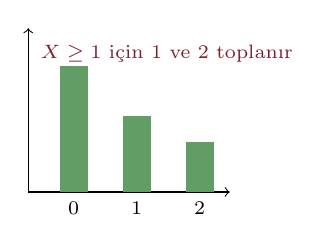
\begin{tikzpicture}[scale=0.8, every node/.style={font=\scriptsize}]
            \draw[->] (0.4,0.4) -- (0.4,3.0);
            \draw[->] (0.4,0.4) -- (3.6,0.4);
            \fill[probExampleGreen!75] (0.9,0.4) rectangle (1.35,2.4);
            \fill[probExampleGreen!75] (1.9,0.4) rectangle (2.35,1.6);
            \fill[probExampleGreen!75] (2.9,0.4) rectangle (3.35,1.2);
            \node[below] at (1.12,0.4) {0};
            \node[below] at (2.12,0.4) {1};
            \node[below] at (3.12,0.4) {2};
            \node[text=probSolutionBurgundy] at (2.6,2.6) {$X\ge1$ için 1 ve 2 toplanır};
        \end{tikzpicture}
    }
\end{questionworkspace}
\end{frame}

\begin{frame}[shrink=8]{Soru 10: Vardiya Başına Robot Arıza Sayısı Çözümü}
\small
\begin{solutionblock}{Adım 1: İstenen olayı PMF üzerinden yaz}
    ``En az bir arıza'' demek
    \[
    X \ge 1
    \]
    olayıdır. PMF verildiği için ilgili değerlerin olasılıklarını toplayabiliriz:
    \[
    P(X \ge 1)=P(X=1)+P(X=2)
    \]
\end{solutionblock}

\begin{solutionblock}{Adım 2: Olasılıkları topla}
    \[
    P(X \ge 1)=0.30+0.20=0.50
    \]
    İstersek tümleyenle de kontrol edebiliriz:
    \[
    P(X \ge 1)=1-P(X=0)=1-0.50=0.50
    \]
\end{solutionblock}

\begin{resultblock}{Yorum}
    İki farklı yol aynı sonuca ulaşıyor. PMF sorularında hem doğrudan toplama hem de tümleyen kullanımı önemli bir kontrol aracıdır.
\end{resultblock}
\end{frame}

\begin{frame}[t]{Soru 11: Uyarı Sayısı İçin PMF Kalibrasyonu}
\scriptsize
\begin{questionworkspace}
    Bir SMT kart üretim hattında, tek bir problemli kontrol kartı üretim boyunca üç aşamada inceleniyor: \textbf{otomatik optik inceleme (AOI)}, \textbf{lehim kontrolü} ve \textbf{son doğrulama}. Bu üç aşama boyunca oluşan \textbf{kritik süreç uyarısı sayısı} $X$, yalnızca $0,1,2,3$ değerlerini alıyor. Kalite ekibi bu sayıyı modellemek için ilk taslak olarak
    \[
    f(x)=c(x^2+4), \qquad x=0,1,2,3
    \]
    fonksiyonunu öneriyor.

    \vspace{0.15cm}
    Bu modelin geçerli bir olasılık kütle fonksiyonu olabilmesi için sabit $c$ değerini bulunuz.
    \setquestionvisual{
        \centering
        \begin{tabular}{@{}ccccc@{}}
            \toprule
            $x$ & 0 & 1 & 2 & 3 \\ \midrule
            $x^2+4$ & 4 & 5 & 8 & 13 \\ \bottomrule
        \end{tabular}
    }
\end{questionworkspace}
\end{frame}

\begin{frame}[shrink=8]{Soru 11: Uyarı Sayısı İçin PMF Kalibrasyonu Çözümü}
\scriptsize
\begin{solutionblock}{Adım 1: PMF'nin toplamı 1 olmalıdır}
    Geçerli bir PMF için tüm olasılıkların toplamı 1'dir:
    \[
    \sum_{x=0}^{3} c(x^2+4)=1
    \]
\end{solutionblock}

\begin{solutionblock}{Adım 2: Toplamı açıkça hesapla}
    \[
    c\big[(0^2+4)+(1^2+4)+(2^2+4)+(3^2+4)\big]=1
    \]
    \[
    c(4+5+8+13)=1
    \]
    \[
    30c=1 \qquad \Rightarrow \qquad c=\frac{1}{30}
    \]
\end{solutionblock}

\begin{resultblock}{Yorum}
    Sabit $c$, dağılımı normalize eden katsayıdır. PMF sorularında ilk kontrol her zaman toplamın 1 olup olmadığıdır.
\end{resultblock}
\end{frame}

\begin{frame}[t]{Soru 12: İlk Kritik Alarm Dakikası için Rekürsif PMF}
\scriptsize
\begin{questionworkspace}
    Bir izleme yazılımında ilk kritik alarmın $x$'inci dakikada gelme olasılığı $X$ ile modelleniyor. Telemetri raporuna göre alarmın bir sonraki dakikaya sarkma olasılığı, her adımda bir öncekinin üçte biri kadar:
    \[
    P(X=x+1)=\frac{1}{3}P(X=x), \qquad x \ge 1
    \]

    \vspace{0.15cm}
    $P(X=x)$ için kapalı form ifadeyi bulunuz.
    \setquestionvisual{
        \centering
        \begin{tikzpicture}[scale=0.90, every node/.style={font=\scriptsize}]
            \node[qgreen, minimum width=1.2cm] (x1) at (0.6,1.8) {$x=1$};
            \node[qgreen, minimum width=1.2cm] (x2) at (2.2,1.8) {$x=2$};
            \node[qgreen, minimum width=1.2cm] (x3) at (3.8,1.8) {$x=3$};
            \draw[qline] (x1) -- node[above] {$\times \tfrac{1}{3}$} (x2);
            \draw[qline] (x2) -- node[above] {$\times \tfrac{1}{3}$} (x3);
            \node[text=probInfoGray] at (2.2,0.8) {geometrik azalma};
        \end{tikzpicture}
    }
\end{questionworkspace}
\end{frame}

\begin{frame}{Soru 12: İlk Kritik Alarm Dakikası için Rekürsif PMF Çözümü I}
\scriptsize
\begin{solutionblock}{Adım 1: Rekürsif yapıdan genel biçimi tahmin et}
    $P(X=1)=a$ diyelim. Her yeni terim bir öncekinin $\frac{1}{3}$ katı olduğundan
    \[
    P(X=x)=a\left(\frac{1}{3}\right)^{x-1}, \qquad x \ge 1
    \]
    biçiminde geometrik bir dizi elde ederiz.
\end{solutionblock}
\begin{infoblock}{Geçiş Notu}
    Artık dizi biçimini bulduk. Sıradaki iş, bu olasılıkların toplamını 1'e eşitleyip $a$ sabitini belirlemektir.
\end{infoblock}
\end{frame}

\begin{frame}{Soru 12: İlk Kritik Alarm Dakikası için Rekürsif PMF Çözümü II}
\scriptsize
\begin{solutionblock}{Adım 2: Normalizasyon ile $a$ sabitini bul}
    \[
    1=\sum_{x=1}^{\infty} a\left(\frac{1}{3}\right)^{x-1}
    =a\sum_{x=0}^{\infty}\left(\frac{1}{3}\right)^x
    =a\frac{1}{1-\frac{1}{3}}
    =\frac{3a}{2}
    \]
    Buradan
    \[
    a=\frac{2}{3}
    \]
    bulunur.
\end{solutionblock}

\begin{resultblock}{Sonuç}
    Kapalı form:
    \[
    P(X=x)=\frac{2}{3^x}, \qquad x=1,2,3,\ldots
    \]
    olur. Rekürsif verilen PMF'lerde temel fikir, önce dizinin biçimini kurup sonra toplamı 1'e eşitlemektir.
\end{resultblock}
\end{frame}

\begin{frame}[t]{Soru 13: Hata Kümesi Uzunluğu Modelinde Normalizasyon}
\scriptsize
\begin{questionworkspace}
    Bir haberleşme kanalında tek bir hata kümesinin uzunluğu $X$ için aşağıdaki ayrık model öneriliyor:
    \[
    f(x)=c\frac{(-1)^{x-1}}{x}q^x, \qquad x \ge 1,\quad q\in(-1,0)
    \]
    Bu modelin geçerli bir PMF olması için $c$ sabitini bulunuz.
    \setquestionvisual{
        \centering
        \begin{tabular}{@{}lc@{}}
            \toprule
            $x$ & terim \\ \midrule
            1 & $cq$ \\
            2 & $-\frac{cq^2}{2}$ \\
            3 & $\frac{cq^3}{3}$ \\ \bottomrule
        \end{tabular}
    }
\end{questionworkspace}
\end{frame}

\begin{frame}{Soru 13: Hata Kümesi Uzunluğu Modelinde Normalizasyon Çözümü I}
\scriptsize
\begin{solutionblock}{Adım 1: Tüm olasılıkların toplamını 1'e eşitle}
    Geçerli bir PMF için
    \[
    1=c\sum_{x=1}^{\infty}\frac{(-1)^{x-1}}{x}q^x
    \]
    yazılır.
\end{solutionblock}
\begin{infoblock}{Geçiş Notu}
    Bu seriyi kapalı biçimde toplayabilirsek normalizasyon sabiti doğrudan ortaya çıkar.
\end{infoblock}
\end{frame}

\begin{frame}{Soru 13: Hata Kümesi Uzunluğu Modelinde Normalizasyon Çözümü II}
\scriptsize
\begin{columns}[T,onlytextwidth]
    \begin{column}{0.56\textwidth}
        
        \begin{solutionblock}{Adım 2: Standart seri formülünü açıkça kullan}
            Burada doğrudan kullanılan temel seri formülü şudur:
            \[
            -\ln(1-t)=\sum_{x=1}^{\infty}\frac{t^x}{x},
            \qquad |t|<1
            \]
            Bu soruda $q\in(-1,0)$ olduğundan $u=-q\in(0,1)$ yazabiliriz.
            \[
            \sum_{x=1}^{\infty}\frac{(-1)^{x-1}}{x}q^x
            =-\sum_{x=1}^{\infty}\frac{u^x}{x}
            \]
            olur. Standart formülde $t=u$ koyarsak
            \[
            \sum_{x=1}^{\infty}\frac{u^x}{x}=-\ln(1-u)
            \]
            elde edilir. Dolayısıyla sonuç
            \[
            \sum_{x=1}^{\infty}\frac{(-1)^{x-1}}{x}q^x
            =\ln(1-u)=\ln(1+q) olur.
            \]
        \end{solutionblock}
    \end{column}
    \begin{column}{0.40\textwidth}
        \begin{infoblock}{Benzerlik Neden Var?}
            Bu seri logaritmanın Taylor serisine benzer; çünkü aslında o serinin dönüştürülmüş halidir.

            \vspace{0.15cm}
            Yeni bir formül ezberlemiyoruz; yalnızca bilinen
            \[
            -\ln(1-t)=\sum_{x=1}^{\infty}\frac{t^x}{x}
            \]
            serisinde $t=-q$ dönüşümünü kullanıyoruz.
        \end{infoblock}

        \begin{resultblock}{Sonuç}
            \[
            c\,\ln(1+q)=1
            \qquad \Rightarrow \qquad
            c=\frac{1}{\ln(1+q)}
            \]
        \end{resultblock}
    \end{column}
\end{columns}
\end{frame}

\begin{frame}[t]{Soru 14: Tekrar Gönderilen Mesaj Sayısı}
\scriptsize
\begin{columns}[T,onlytextwidth]
    \begin{column}{0.70\textwidth}
        \begin{exampleblock}{Soru}
            \setlength{\abovedisplayskip}{3pt}
            \setlength{\belowdisplayskip}{3pt}
            \setlength{\abovedisplayshortskip}{2pt}
            \setlength{\belowdisplayshortskip}{2pt}
            \setlength{\itemsep}{0.2em}

            Bir bilgisayar sistemi bir mesaj gönderdiğinde, bazı mesajlar ilk denemede karşı tarafa ulaşmaz. Bu durumda sistem aynı mesajı tekrar göndermeyi dener.

            \vspace{0.15cm}
            Bir saniye içinde oluşan \textbf{tekrar gönderim sayısı} $X$ ile gösterilsin. Yani:
            \begin{itemize}
                \item $X=0$: o saniyede hiç tekrar gönderim olmadı,
                \item $X=1$: bir kez tekrar gönderim oldu,
                \item $X=2$: iki kez tekrar gönderim oldu.
            \end{itemize}

            Bu değişken için olasılık modeli aşağıdaki gibi veriliyor.
            \[
            f(x)=c\frac{2^x}{x!}, \qquad x=0,1,2,\ldots
            \]
            

            \vspace{0.15cm}
            \begin{enumerate}
                \item Bu modelin geçerli bir olasılık kütle fonksiyonu olması için $c$ sabitini bulunuz.
                \item Bir saniyede \textbf{en az iki tekrar gönderim} olma olasılığını, yani $P(X \ge 2)$ değerini hesaplayınız.
            \end{enumerate}
        \end{exampleblock}
    \end{column}
    \begin{column}{0.29\textwidth}
        \centering
        \begin{tabular}{@{}ccccc@{}}
            \toprule
            $x$ & 0 & 1 & 2 & 3 \\ \midrule
            $\frac{2^x}{x!}$ & 1 & 2 & 2 & $\frac{4}{3}$ \\ \bottomrule
        \end{tabular}

        \vspace{0.15cm}
        {\scriptsize seri yapısı $\rightarrow e^2$}
    \end{column}
\end{columns}
\end{frame}

\begin{frame}[t]{Soru 14: Tekrar Gönderilen Mesaj Sayısı Çözümü I}
\scriptsize
\begin{columns}[T,onlytextwidth]
    \begin{column}{0.48\textwidth}
        \begin{solutionblock}{Adım 1a: Toplamı 1'e eşitle}
            Geçerli bir PMF'de tüm olasılıkların toplamı 1 olmalıdır. Bu yüzden
            \[
            1=\sum_{x=0}^{\infty} c\frac{2^x}{x!}
            =c\sum_{x=0}^{\infty}\frac{2^x}{x!}
            \]
            Buradaki kritik nokta,
            \[
            \sum_{x=0}^{\infty}\frac{2^x}{x!}
            \]
            serisinin hangi bilinen fonksiyona ait olduğunu görmektir.
        \end{solutionblock}
    \end{column}
    \begin{column}{0.48\textwidth}
        \begin{solutionblock}{Adım 1b: Neden $e^2$?}
            Üstel fonksiyonun temel seri açılımı
            \[
            e^t=\sum_{x=0}^{\infty}\frac{t^x}{x!}
            =1+t+\frac{t^2}{2!}+\cdots
            \]
            şeklindedir. Bu formülde $t=2$ yazarsak
            \[
            e^2=\sum_{x=0}^{\infty}\frac{2^x}{x!}
            =1+2+\frac{2^2}{2!}+\cdots
            \]
            olur. Dolayısıyla
            \[
            1=c\,e^2
            \qquad \Rightarrow \qquad
            c=e^{-2}
            \]
        \end{solutionblock}
    \end{column}
\end{columns}
\begin{infoblock}{Geçiş Notu}
    Model artık geçerli hale geldi. Şimdi bu sabiti kullanarak ``bir saniyede en az iki tekrar gönderim'' olasılığını hesaplayacağız.
\end{infoblock}
\end{frame}

\begin{frame}{Soru 14: Tekrar Gönderilen Mesaj Sayısı Çözümü II}
\scriptsize
\begin{solutionblock}{Adım 2: İstenen olasılığı tümleyenle hesapla}
    ``En az iki'' demek, 0 ve 1 durumlarını dışarıda bırakmak demektir. Bu nedenle
    \[
    P(X \ge 2)=1-P(X=0)-P(X=1)
    \]
    \[
    =1-c\frac{2^0}{0!}-c\frac{2^1}{1!}
    =1-c-2c
    =1-3e^{-2}
    \]
    \[
    P(X \ge 2)\approx 1-3(0.1353)\approx 0.594
    \]
\end{solutionblock}

\begin{resultblock}{Yorum}
    Bu soru ağ teknolojisi bilmeden de okunabilir: aslında yaptığımız şey, ``bir zaman aralığında olay kaç kez tekrar etti?'' sorusunu modellemektir. Önce modeli geçerli hale getiriyoruz, sonra istenen sayım olasılığını buluyoruz.
\end{resultblock}
\end{frame}

\begin{frame}[t]{Soru 15: Numune Çekmecesinden Seçilen Kırmızı Test Pulları}
\scriptsize
\begin{questionworkspace}
    Bir kalite laboratuvarındaki numune çekmecesinde 6 kırmızı, 5 beyaz ve 8 mavi test pulu vardır. Deney seti hazırlamak için geri koymadan rastgele 4 pul seçiliyor.

    \vspace{0.15cm}
    Seçilen kırmızı pul sayısını gösteren rastgele değişken $X$ olsun.

    \vspace{0.15cm}
    \begin{enumerate}
        \item $X$'in olasılık kütle fonksiyonunu bulunuz.
        \item En az bir kırmızı pul çekilmesi olasılığını hesaplayınız.
    \end{enumerate}
    \setquestionvisual{
        \centering
        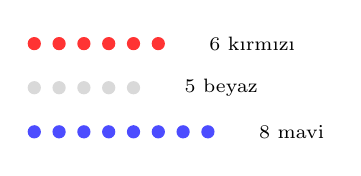
\begin{tikzpicture}[scale=0.7]
            \foreach \i in {0,...,5}{\fill[red!80] (0.45*\i,2.2) circle (0.12);}
            \foreach \i in {0,...,4}{\fill[black!15] (0.45*\i,1.4) circle (0.12);}
            \foreach \i in {0,...,7}{\fill[blue!70] (0.45*\i,0.6) circle (0.12);}
            \node[anchor=west,font=\scriptsize] at (3.0,2.2) {6 kırmızı};
            \node[anchor=west,font=\scriptsize] at (2.55,1.4) {5 beyaz};
            \node[anchor=west,font=\scriptsize] at (3.9,0.6) {8 mavi};
        \end{tikzpicture}
    }
\end{questionworkspace}
\end{frame}

\begin{frame}{Soru 15: Numune Çekmecesinden Seçilen Kırmızı Test Pulları Çözümü I}
\scriptsize
\begin{solutionblock}{Adım 1: Dağılımın türünü tanı}
    Geri koymadan seçim yapıldığı için bu soru \textbf{hipergeometrik} yapıdadır. Toplam 19 pulun 6'sı kırmızı, 13'ü kırmızı dışıdır. Bu nedenle
    \[
    f(x)=P(X=x)=\frac{\binom{6}{x}\binom{13}{4-x}}{\binom{19}{4}},
    \qquad x=0,1,2,3,4
    \]
    elde edilir.
\end{solutionblock}
\begin{infoblock}{Geçiş Notu}
    PMF kurulduktan sonra ikinci istek doğrudan bu dağılım üzerinden ya da tümleyenle hesaplanabilir.
\end{infoblock}
\end{frame}

\begin{frame}{Soru 15: Numune Çekmecesinden Seçilen Kırmızı Test Pulları Çözümü II}
\scriptsize
\begin{solutionblock}{Adım 2: En az bir kırmızıyı tümleyenle hesapla}
    \[
    P(X \ge 1)=1-P(X=0)
    \]
    \[
    =1-\frac{\binom{6}{0}\binom{13}{4}}{\binom{19}{4}}
    =1-\frac{\binom{13}{4}}{\binom{19}{4}}
    =1-\frac{715}{3876}
    =\frac{3161}{3876}\approx 0.8155
    \]
\end{solutionblock}

\begin{resultblock}{Yorum}
    En az bir kırmızı pul görme olasılığı oldukça yüksektir. Bu tip sayım sorularında ``istenen olay'' yerine çoğu zaman ``istenmeyen olay''ı hesaplamak daha kısadır.
\end{resultblock}
\end{frame}

\begin{frame}[t]{Soru 16: Sevkiyattan Alınan Arızalı Dizüstü Sayısı}
\scriptsize
\begin{questionworkspace}
    20 dizüstü bilgisayardan oluşan bir sevkiyatta 3 bilgisayar arızalıdır. Bir okul bu sevkiyattan rastgele 2 bilgisayar satın alıyor.

    \vspace{0.15cm}
    Satın alınan arızalı bilgisayar sayısını gösteren rastgele değişken $X$ için PMF'yi bulunuz.
    \setquestionvisual{
        \centering
        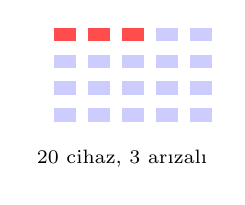
\begin{tikzpicture}[scale=0.62]
            \foreach \r in {0,...,3}{
                \foreach \c in {0,...,4}{
                    \pgfmathtruncatemacro{\n}{5*\r+\c+1}
                    \ifnum\n<4
                        \fill[red!70] (\c*0.7,-\r*0.55) rectangle ++(0.45,0.28);
                    \else
                        \fill[blue!20] (\c*0.7,-\r*0.55) rectangle ++(0.45,0.28);
                    \fi
                }
            }
            \node[font=\scriptsize] at (1.4,-2.4) {20 cihaz, 3 arızalı};
        \end{tikzpicture}
    }
\end{questionworkspace}
\end{frame}

\begin{frame}{Soru 16: Sevkiyattan Alınan Arızalı Dizüstü Sayısı Çözümü I}
\scriptsize
\begin{solutionblock}{Adım 1: Dağılımın yapısını kur}
    Geri koyma yoktur ve iki seçim sabit büyüklükte bir kitleden yapılmaktadır. Bu nedenle $X$ hipergeometrik dağılıma sahiptir:
    \[
    f(x)=\frac{\binom{3}{x}\binom{17}{2-x}}{\binom{20}{2}},
    \qquad x=0,1,2
    \]
\end{solutionblock}
\begin{infoblock}{Geçiş Notu}
    Model kurulduktan sonra sıra, $x=0,1,2$ için bu formülü sayısal olarak değerlendirmeye gelir.
\end{infoblock}
\end{frame}

\begin{frame}{Soru 16: Sevkiyattan Alınan Arızalı Dizüstü Sayısı Çözümü II}
\scriptsize
\begin{solutionblock}{Adım 2: Olasılık değerlerini hesapla}
    \[
    f(0)=\frac{\binom{3}{0}\binom{17}{2}}{\binom{20}{2}}=\frac{136}{190}
    \]
    \[
    f(1)=\frac{\binom{3}{1}\binom{17}{1}}{\binom{20}{2}}=\frac{51}{190}
    \]
    \[
    f(2)=\frac{\binom{3}{2}\binom{17}{0}}{\binom{20}{2}}=\frac{3}{190}
    \]
\end{solutionblock}

\begin{resultblock}{Yorum}
    En yüksek olasılık, okulun iki sağlam bilgisayar almasıdır. Küçük örneklemli sevkiyat sorularında hipergeometrik model doğal seçimdir.
\end{resultblock}
\end{frame}

\begin{frame}[t]{Soru 17: Dört Satışta Yan Hava Yastıklı Araç Sayısı}
\scriptsize
\begin{questionworkspace}
    Bir otomobil galerisi sattığı araçların yaklaşık \%50'sini yan hava yastıklı paketle satmaktadır. Satılan sonraki 4 araç için her satışın birbirinden bağımsız olduğu varsayılıyor.

    \vspace{0.15cm}
    $X$, bu 4 araç içinde yan hava yastığı bulunan araç sayısı olsun.

    \vspace{0.15cm}
    $f(x)=P(X=x)$ PMF'sini yazınız.
    \setquestionvisual{
        \centering
        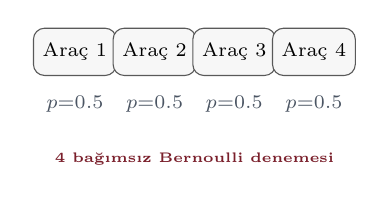
\begin{tikzpicture}[scale=0.88, every node/.style={font=\scriptsize}]
            \foreach \i/\x in {1/0.55,2/1.7,3/2.85,4/4.0}{
                \node[qbox, minimum width=0.9cm, minimum height=0.6cm] at (\x,2.0) {Araç~\i};
                \node[text=probInfoGray] at (\x,1.25) {$p{=}0.5$};
            }
            \node[font=\tiny\bfseries, text=probSolutionBurgundy, text width=4.0cm, align=center] at (2.275,0.45) {4 bağımsız Bernoulli denemesi};
        \end{tikzpicture}
    }
\end{questionworkspace}
\end{frame}

\begin{frame}[shrink=8]{Soru 17: Dört Satışta Yan Hava Yastıklı Araç Sayısı Çözümü}
\scriptsize
\begin{solutionblock}{Adım 1: Binom modeli olduğunu fark et}
    Sabit sayıda deneme vardır ($n=4$), her denemede başarı olasılığı aynıdır ($p=0.5$) ve denemeler bağımsız kabul edilir. Dolayısıyla
    \[
    X \sim Bin(4,0.5)
    \]
    olur.
\end{solutionblock}

\begin{solutionblock}{Adım 2: Binom PMF'yi yaz}
    \[
    f(x)=P(X=x)=\binom{4}{x}(0.5)^x(0.5)^{4-x}
    \]
    \[
    =\frac{\binom{4}{x}}{16},
    \qquad x=0,1,2,3,4
    \]
\end{solutionblock}

\begin{resultblock}{Yorum}
    Bu soru daha sonra CDF hesabında da kullanılacaktır. Önce doğru PMF'yi kurmak, birikimli olasılık hesaplarını çok kolaylaştırır.
\end{resultblock}
\end{frame}

\begin{frame}[t]{Soru 18: İşlemci Hata PMF'sinden Koşullu Olasılık}
\scriptsize
\begin{questionworkspace}
    $X$, bir işlemcide gözlenen hata sayısını göstersin:
    \[
    P(X=x)=k(4-x), \qquad x\in\{0,1,2,3\}
    \]

    \vspace{0.15cm}
    En az bir hata olduğu biliniyorsa, tam olarak 2 hata bulunması olasılığı nedir?
    \setquestionvisual{
        \centering
        \begin{tabular}{@{}ccccc@{}}
            \toprule
            $x$ & 0 & 1 & 2 & 3 \\ \midrule
            $4-x$ & 4 & 3 & 2 & 1 \\ \bottomrule
        \end{tabular}

        \vspace{0.15cm}
        {\scriptsize koşul: $X\ge1$}
    }
\end{questionworkspace}
\end{frame}

\begin{frame}[shrink=8]{Soru 18: İşlemci Hata PMF'sinden Koşullu Olasılık Çözümü}
\scriptsize
\begin{solutionblock}{Adım 1: Önce eksik sabiti bul}
    PMF toplamı 1 olmalıdır:
    \[
    k(4+3+2+1)=1
    \qquad \Rightarrow \qquad
    10k=1
    \qquad \Rightarrow \qquad
    k=\frac{1}{10}
    \]
\end{solutionblock}

\begin{solutionblock}{Adım 2: Koşullu olasılık oranını kur}
    \[
    P(X=2)=\frac{2}{10}, \qquad P(X\ge 1)=1-P(X=0)=1-\frac{4}{10}=\frac{6}{10}
    \]
    Bu yüzden
    \[
    P(X=2 \mid X\ge 1)=\frac{P(X=2)}{P(X\ge 1)}
    =\frac{2/10}{6/10}=\frac{1}{3}
    \]
\end{solutionblock}

\begin{resultblock}{Yorum}
    Koşul, örnek uzayı ``en az bir hata'' kümesine daraltır. Bu daraltmadan sonra iki hata olayı, yeni evrende üçte birlik paya sahiptir.
\end{resultblock}
\end{frame}

\begin{frame}[t]{Soru 19: İki Bakım Ekibinin Daha Geç Tamamlanma Günü}
\scriptsize
\begin{questionworkspace}
    İki bağımsız bakım ekibi, benzer büyüklükte iki arızaya gönderiliyor. Her ekibin işi tamamlama günü, 1 ile 6 gün arasında eşit olasılıkla dağılan ayrık değişkenlerle modelleniyor.

    \vspace{0.15cm}
    İlk ekibin tamamlama günü $X$, ikinci ekibin tamamlama günü $Y$ olsun.

    \vspace{0.15cm}
    \[
    Z=\max(X,Y)
    \]
    ortak sistemin yeniden devreye alınabileceği günü gösteriyor. $Z$ için PMF'yi bulunuz.
    \setquestionvisual{
        \centering
        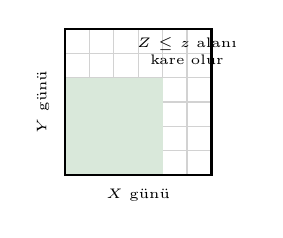
\begin{tikzpicture}[scale=0.62]
            \draw[step=0.5, gray!35] (0,0) grid (3,3);
            \draw[fill=probExampleGreen!18, draw=none] (0,0) rectangle (2,2);
            \draw[thick] (0,0) rectangle (3,3);
            \node[font=\tiny] at (1.5,-0.40) {$X$ günü};
            \node[font=\tiny, rotate=90] at (-0.45,1.5) {$Y$ günü};
            \node[font=\tiny, align=center, text width=1.5cm] at (2.5,2.55) {$Z\le z$ alanı \\ kare olur};
        \end{tikzpicture}
    }
\end{questionworkspace}
\end{frame}

\begin{frame}[shrink=8]{Soru 19: İki Bakım Ekibinin Daha Geç Tamamlanma Günü Çözümü}
\scriptsize
\begin{solutionblock}{Adım 1: Önce CDF benzeri bir yardımcı ifade kur}
    $Z\le z$ olması için hem $X\le z$ hem de $Y\le z$ olmalıdır. Bağımsızlıktan
    \[
    P(Z\le z)=P(X\le z,\;Y\le z)=\left(\frac{z}{6}\right)^2,
    \qquad z=1,2,\ldots,6
    \]
    elde edilir.
\end{solutionblock}

\begin{solutionblock}{Adım 2: Ardışık fark alarak PMF'ye geç}
    \[
    P(Z=z)=P(Z\le z)-P(Z\le z-1)
    \]
    \[
    =\frac{z^2-(z-1)^2}{36}
    =\frac{2z-1}{36},
    \qquad z=1,2,\ldots,6
    \]
\end{solutionblock}

\begin{resultblock}{Yorum}
    Maksimum gibi türetilmiş değişkenlerde doğrudan PMF yazmak zor olabilir. Önce $P(Z\le z)$ türü bir ifade kurmak genellikle en temiz yoldur.
\end{resultblock}
\end{frame}

\begin{frame}[t]{Soru 20: Üçüncü Başarısızlığa Kadar Test Edilen Bileşen Sayısı}
\scriptsize
\begin{questionworkspace}
    Bir kalite kontrol sürecinde bileşenler bağımsız olarak test ediliyor.

    \vspace{0.15cm}
    Testi geçme olasılığı $0.8$, başarısız olma olasılığı $0.2$'dir. Tam olarak 3 başarısızlık kaydedilene kadar teste devam ediliyor.

    \vspace{0.15cm}
    Toplam test edilen bileşen sayısını gösteren rastgele değişken $N$ için
    \begin{enumerate}
        \item genel PMF ifadesini,
        \item $P(N=5)$ olasılığını
    \end{enumerate}
    bulunuz.
    \setquestionvisual{
        \centering
        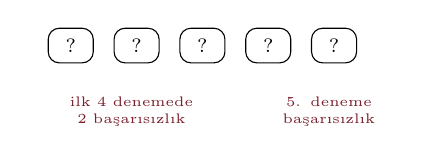
\begin{tikzpicture}[scale=0.88, every node/.style={font=\scriptsize}]
            \foreach \i/\x in {1/0.5,2/1.45,3/2.4,4/3.35,5/4.3}{
                \draw[rounded corners] (\x,1.55) rectangle ++(0.65,0.50);
                \node at (\x+0.325,1.80) {?};
            }
            \node[font=\tiny, text=probSolutionBurgundy, text width=2.4cm, align=center] at (1.7,0.85) {ilk 4 denemede \\ 2 başarısızlık};
            \node[font=\tiny, text=probSolutionBurgundy, text width=2.0cm, align=center] at (4.55,0.85) {5. deneme \\ başarısızlık};
        \end{tikzpicture}
    }
\end{questionworkspace}
\end{frame}

\begin{frame}[shrink=8]{Soru 20: Üçüncü Başarısızlığa Kadar Test Edilen Bileşen Sayısı Çözümü}
\scriptsize
\begin{solutionblock}{Adım 1: Üçüncü başarısızlığın geliş anını model kur}
    Üçüncü başarısızlığın $n$'inci denemede gelmesi için ilk $n-1$ denemede tam 2 başarısızlık, son denemede de bir başarısızlık olmalıdır. Bu nedenle
    \[
    P(N=n)=\binom{n-1}{2}(0.2)^3(0.8)^{n-3},
    \qquad n=3,4,5,\ldots
    \]
    yazılır.
\end{solutionblock}

\begin{solutionblock}{Adım 2: İstenen özel değeri hesapla}
    \[
    P(N=5)=\binom{4}{2}(0.2)^3(0.8)^2
    \]
    \[
    =6 \times 0.008 \times 0.64 = 0.03072
    \]
\end{solutionblock}

\begin{resultblock}{Yorum}
    Negatif binom yapısında odak, toplam başarı sayısı değil belirli sayıda başarısızlığın hangi denemede tamamlandığıdır.
\end{resultblock}
\end{frame}

% ------------------------------------------------------------------
% MILESTONE 8: BİRİKİMLİ DAĞILIM FONKSİYONU (CDF)
% ------------------------------------------------------------------
\begin{frame}[fragile]
    \frametitle[CDF]{Tekrar 8: Birikimli Dağılım Fonksiyonu (CDF)}
    \small
    \begin{block}{Tanım}
        Rastgele değişken $X$'in belirli bir $x$ değerine eşit veya daha küçük olma olasılıklarının toplamıdır:
        \[
        F(x) = P(X \le x) = \sum_{t \le x} f(t), \qquad -\infty < x < \infty
        \]
    \end{block}

    \begin{columns}[T]
        \begin{column}{0.48\textwidth}
            \begin{infoblock}{Kumbara Mantığı}
                \begin{itemize}
                    \item CDF, soldan sağa doğru olasılıkları \textbf{üst üste ekler}.
                    \item Hiçbir zaman azalmaz (basamak fonksiyonu).
                    \item $F(-\infty) = 0$, \; $F(\infty) = 1$.
                \end{itemize}
            \end{infoblock}
        \end{column}
        \begin{column}{0.48\textwidth}
            \begin{block}{Aralık Olasılığı}
                CDF biliniyorsa:
                \[
                P(a < X \le b) = F(b) - F(a)
                \]
                Geriye dönüş:
                \[
                f(x) = F(x) - F(x^{-})
                \]
            \end{block}
        \end{column}
    \end{columns}
\end{frame}

\begin{frame}[t]{Soru 21: CDF ile Ağ Cihazı Paket Kaybını Okumak}
\small
\begin{questionworkspace}
    Bir ağ cihazında günlük paket kaybı sayısı için
    \[
    \begin{aligned}
    P(X=0)&=0.20 \\
    P(X=1)&=0.50 \\
    P(X=2)&=0.30
    \end{aligned}
    \]
    veriliyor.

    \vspace{0.15cm}
    \(F(1)=P(X\le 1)\) ve \(P(1<X\le 2)\) değerlerini bulunuz.
    \setquestionvisual{
        \centering
        \begin{tabular}{@{}cccc@{}}
            \toprule
            $x$ & 0 & 1 & 2 \\ \midrule
            $P(X=x)$ & 0.20 & 0.50 & 0.30 \\
            $F(x)$ & 0.20 & 0.70 & 1.00 \\ \bottomrule
        \end{tabular}
    }
\end{questionworkspace}
\end{frame}

\begin{frame}[shrink=8]{Soru 21: CDF ile Ağ Cihazı Paket Kaybını Okumak Çözümü}
\small
\begin{solutionblock}{Adım 1: Birikimli olasılığı hesapla}
    \[
    F(1)=P(X=0)+P(X=1)=0.20+0.50=0.70
    \]
    Çünkü CDF, 1'e kadar olan tüm olasılıkları toplar.
\end{solutionblock}

\begin{solutionblock}{Adım 2: Aralık olasılığını CDF farkı ile bul}
    Burada $X$ en fazla 2 değerine kadar gidebildiği için $F(2)=1$'dir. O halde
    \[
    P(1<X\le 2)=F(2)-F(1)=1-0.70=0.30
    \]
\end{solutionblock}

\begin{resultblock}{Yorum}
    CDF, tek tek olasılık toplamayı sistematik hale getirir. Özellikle aralık olasılıklarında fark alma yöntemi büyük kolaylık sağlar.
\end{resultblock}
\end{frame}

\begin{frame}[t]{Soru 22: Galeri Satışlarında En Fazla İki Yan Hava Yastıklı Araç}
\scriptsize
\begin{questionworkspace}
    17. sorudaki binom modele göre, satılan sonraki 4 aracın en fazla 2 tanesinde yan hava yastığı bulunması olasılığı nedir?

    \vspace{0.15cm}
    Yani
    \[
    F(2)=P(X\le 2)
    \]
    değerini bulunuz.
    \setquestionvisual{
        \centering
        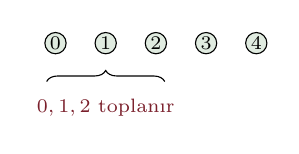
\begin{tikzpicture}[scale=0.75, every node/.style={font=\scriptsize}]
            \foreach \x/\lbl in {0.5/0,1.35/1,2.2/2,3.05/3,3.9/4}{
                \draw[fill=probExampleGreen!15] (\x,1.2) circle (0.18);
                \node at (\x,1.2) {\lbl};
            }
            \draw[decorate, decoration={brace, amplitude=4pt}] (0.35,0.55) -- (2.35,0.55);
            \node[text=probSolutionBurgundy] at (1.35,0.1) {$0,1,2$ toplanır};
        \end{tikzpicture}
    }
\end{questionworkspace}
\end{frame}

\begin{frame}{Soru 22: Galeri Satışlarında En Fazla İki Yan Hava Yastıklı Araç Çözümü I}
\scriptsize
\begin{solutionblock}{Adım 1: İlgili değerleri topla}
    17. soruda
    \[
    X\sim Bin(4,0.5)
    \]
    bulunmuştu. Bu nedenle
    \[
    F(2)=\sum_{x=0}^{2} \binom{4}{x}(0.5)^x(0.5)^{4-x}
    \]
    yazılır.
\end{solutionblock}
\begin{infoblock}{Geçiş Notu}
    Bu toplamı doğrudan açabiliriz; ortak $(0.5)^4$ çarpanı işlemi belirgin biçimde sadeleştirir.
\end{infoblock}
\end{frame}

\begin{frame}{Soru 22: Galeri Satışlarında En Fazla İki Yan Hava Yastıklı Araç Çözümü II}
\scriptsize
\begin{solutionblock}{Adım 2: Ortak çarpanı kullanarak sadeleştir}
    \[
    F(2)=\sum_{x=0}^{2}\binom{4}{x}(0.5)^4
    =\frac{\binom{4}{0}+\binom{4}{1}+\binom{4}{2}}{16}
    \]
    \[
    =\frac{1+4+6}{16}=\frac{11}{16}=0.6875
    \]
\end{solutionblock}

\begin{resultblock}{Yorum}
    ``En fazla 2'' türü ifadeler doğrudan CDF düşüncesine karşılık gelir. Bu yüzden binom PMF bulunduğunda, CDF hesapları doğal olarak bir sonraki adımdır.
\end{resultblock}
\end{frame}

\begin{frame}[t]{Soru 23: CDF'den Enerji Ceza Puanına Geçiş}
\scriptsize
\begin{questionworkspace}
    Bir otomatik depoda bir paketin gün içindeki yeniden işleme sayısı $X$ ile gösterilsin. Bu sayının CDF'si
    \[
    F(x)=
    \begin{cases}
    0, & x<1,\\
    0.1, & 1\le x<3,\\
    0.4, & 3\le x<5,\\
    0.8, & 5\le x<7,\\
    1.0, & x\ge 7
    \end{cases}
    \]
    olarak veriliyor.

    Operasyon ekibi enerji ceza puanını \(Y=X^2-10\) olarak tanımlıyor. $Y$'nin PMF'sini bulunuz.
    \setquestionvisual{
        \centering
        \begin{tikzpicture}[scale=0.6, every node/.style={font=\scriptsize}]
            \draw[->] (0,0) -- (4.5,0) node[right] {$x$};
            \draw[->] (0,0) -- (0,3.2) node[above] {$F(x)$};
            \draw[thick] (0.5,0.3) -- (1.4,0.3) -- (1.4,1.0) -- (2.3,1.0) -- (2.3,1.8) -- (3.2,1.8) -- (3.2,2.6) -- (4.0,2.6) -- (4.0,3.0);
            \foreach \x/\lbl in {0.5/1,1.4/3,2.3/5,3.2/7}{
                \draw (\x,0.0) -- (\x,-0.1);
                \node[below] at (\x,0) {\lbl};
            }
        \end{tikzpicture}
    }
\end{questionworkspace}
\end{frame}

\begin{frame}[shrink=8]{Soru 23: CDF'den Enerji Ceza Puanına Geçiş Çözümü}
\scriptsize
\begin{solutionblock}{Adım 1: CDF'deki sıçramalardan PMF'yi çıkar}
    CDF'nin sabit kaldığı yerler yeni olasılık üretmez; sıçrama miktarı ise ilgili noktadaki olasılığı verir:
    \[
    P(X=1)=0.1,\quad P(X=3)=0.3,\quad P(X=5)=0.4,\quad P(X=7)=0.2
    \]
\end{solutionblock}

\begin{solutionblock}{Adım 2: Dönüşümü her değer için uygula}
    \[
    \begin{array}{c|cccc}
    X & 1 & 3 & 5 & 7 \\ \hline
    Y=X^2-10 & -9 & -1 & 15 & 39
    \end{array}
    \]
    Bu nedenle
    \[
    P(Y=-9)=0.1,\;
    P(Y=-1)=0.3,\;
    P(Y=15)=0.4,\;
    P(Y=39)=0.2
    \]
    olur.
\end{solutionblock}

\begin{resultblock}{Yorum}
    CDF'den PMF'ye, oradan da yeni değişkene geçiş aynı akışın parçalarıdır. Önce sıçramaları okuruz, sonra dönüşüm fonksiyonunu uygularız.
\end{resultblock}
\end{frame}

% ------------------------------------------------------------------
% MILESTONE 9: BEKLENEN DEĞER
% ------------------------------------------------------------------
\begin{frame}[fragile]
    \frametitle{Tekrar 9: Beklenen Değer (Matematiksel Beklenti)}
    \begin{columns}[T]
        \begin{column}{0.48\textwidth}
            \begin{block}{Kesikli}
                \[
                \mu = E(X) = \sum_x x\, f(x)
                \]
            \end{block}

            \begin{block}{Sürekli}
                \[
                \mu = E(X) = \int_{-\infty}^{\infty} x\, f(x)\, dx
                \]
            \end{block}
        \end{column}
        \begin{column}{0.48\textwidth}
            \begin{infoblock}{Ne İfade Eder?}
                Dağılımın \textbf{ağırlık merkezi}dir. Deney sonsuz kez tekrarlanırsa, gözlemlerin aritmetik ortalaması bu değere yakınsar.
            \end{infoblock}

            \begin{block}{$g(X)$'in Beklenen Değeri}
                \[
                E[g(X)] = \sum_x g(x)\, f(x)
                \]
                Yeni bir dağılım türetmeye \textbf{gerek yoktur}.
            \end{block}
        \end{column}
    \end{columns}
\end{frame}

\begin{frame}[t]{Soru 24: Sensör Kartında Beklenen Yeniden İşleme Sayısı}
\small
\begin{questionworkspace}
    Bir sensör kartı için yeniden işleme sayısı $X$ aşağıdaki dağılıma sahiptir:
    \[
    \begin{aligned}
    P(X=0)&=0.60 \\
    P(X=1)&=0.30 \\
    P(X=2)&=0.10
    \end{aligned}
    \]

    \vspace{0.15cm}
    Kart başına beklenen yeniden işleme sayısı nedir?
    \setquestionvisual{
        \centering
        \begin{tabular}{@{}cccc@{}}
            \toprule
            $x$ & $P(X=x)$ & $xP(X=x)$ \\ \midrule
            0 & 0.60 & 0 \\
            1 & 0.30 & 0.30 \\
            2 & 0.10 & 0.20 \\ \bottomrule
        \end{tabular}
    }
\end{questionworkspace}
\end{frame}

\begin{frame}[shrink=8]{Soru 24: Sensör Kartında Beklenen Yeniden İşleme Sayısı Çözümü}
\small
\begin{solutionblock}{Adım 1: Beklenen değer formülünü yaz}
    Ayrık durumda
    \[
    E(X)=\sum_x x\,P(X=x)
    \]
    formülünü kullanırız.
\end{solutionblock}

\begin{solutionblock}{Adım 2: Her değeri kendi olasılığı ile çarp}
    \[
    E(X)=0(0.60)+1(0.30)+2(0.10)
    \]
    \[
    =0+0.30+0.20=0.50
    \]
\end{solutionblock}

\begin{resultblock}{Yorum}
    Uzun vadede kart başına ortalama yeniden işleme sayısı 0.50'dir. Bu, her kartın tam yarım kez yeniden işlendiği anlamına gelmez; çok sayıda kart için ortalama davranışı açıklar.
\end{resultblock}
\end{frame}

% ------------------------------------------------------------------
% MILESTONE 10: VARYANS VE STANDART SAPMA
% ------------------------------------------------------------------
\begin{frame}[fragile]
    \frametitle{Tekrar 10: Varyans ve Standart Sapma}
    \scriptsize
    \begin{block}{Tanım}
        Değerlerin ortalamadan sapmalarının karesinin beklenen değeridir:
        \[
        \sigma^2 = Var(X) = E\bigl[(X - \mu)^2\bigr]
        \]
    \end{block}

    \begin{columns}[T]
        \begin{column}{0.48\textwidth}
            \begin{block}{Pratik Formül}
                \[
                \sigma^2 = E(X^2) - \mu^2
                \]
                Hesaplamada daha kolaydır.
            \end{block}
        \end{column}
        \begin{column}{0.48\textwidth}
            \begin{infoblock}{Standart Sapma}
                \[
                \sigma = \sqrt{\sigma^2}
                \]
                Değişkenle \textbf{aynı birime} sahiptir (TL, saat, kg\dots). Sonuçların ortalamadan \textbf{tipik sapmasını} gösterir.
            \end{infoblock}
        \end{column}
    \end{columns}

    \begin{alertblock}{Kritik Nokta}
        Aynı ortalama, aynı yayılım anlamına gelmez; bu farkı varyans ölçer.
    \end{alertblock}
\end{frame}

\begin{frame}[t]{Soru 25: Duruş Sayısında Varyans ve Standart Sapma}
\small
\begin{questionworkspace}
    Bir üretim hücresinde vardiya başına duruş sayısı için
    \[
    \begin{aligned}
    P(X=0)&=0.50 \\
    P(X=1)&=0.30 \\
    P(X=2)&=0.20
    \end{aligned}
    \]
    veriliyor.

    \vspace{0.15cm}
    $Var(X)$ ve $\sigma$ değerlerini bulunuz.
    \setquestionvisual{
        \centering
        \begin{tabular}{@{}cccc@{}}
            \toprule
            $x$ & $P(X=x)$ & $x^2$ \\ \midrule
            0 & 0.50 & 0 \\
            1 & 0.30 & 1 \\
            2 & 0.20 & 4 \\ \bottomrule
        \end{tabular}
    }
\end{questionworkspace}
\end{frame}

\begin{frame}[shrink=8]{Soru 25: Duruş Sayısında Varyans ve Standart Sapma Çözümü}
\small
\begin{solutionblock}{Adım 1: Önce ortalama ve $E(X^2)$ değerlerini bul}
    \[
    E(X)=0(0.50)+1(0.30)+2(0.20)=0.70
    \]
    \[
    E(X^2)=0^2(0.50)+1^2(0.30)+2^2(0.20)=1.10
    \]
\end{solutionblock}

\begin{solutionblock}{Adım 2: Kısa formülle varyansa geç}
    \[
    Var(X)=E(X^2)-[E(X)]^2=1.10-0.49=0.61
    \]
    \[
    \sigma=\sqrt{0.61}\approx 0.78
    \]
\end{solutionblock}

\begin{resultblock}{Yorum}
    Ortalama duruş sayısı 0.70 olsa da süreç her vardiyada tam bu değeri üretmez; standart sapma olan 0.78, duruş sayısının ortalama etrafında ne kadar oynadığını gösterir.
\end{resultblock}
\end{frame}

% ------------------------------------------------------------------
% TEKRAR TABLOSU (BÜYÜK RESİM)
% ------------------------------------------------------------------
\begin{frame}{Tekrar 11: Hafta 2--5 Kavram Haritası}
    \footnotesize
    \centering
    \begin{tikzpicture}[scale=0.75, transform shape, >={Stealth}, thick]
        % Üst satır: Olasılık araçları
        \node[draw=blue!80!black, rounded corners, fill=blue!8, minimum width=2.2cm, minimum height=0.8cm, align=center, font=\scriptsize\bfseries] (kosullu) at (0,3) {Koşullu\\Olasılık};
        \node[draw=blue!80!black, rounded corners, fill=blue!8, minimum width=2.2cm, minimum height=0.8cm, align=center, font=\scriptsize\bfseries] (carpim) at (3.5,3) {Çarpım\\Kuralı};
        \node[draw=blue!80!black, rounded corners, fill=blue!8, minimum width=2.2cm, minimum height=0.8cm, align=center, font=\scriptsize\bfseries] (toplam) at (7,3) {Toplam\\Olasılık};
        \node[draw=blue!80!black, rounded corners, fill=blue!8, minimum width=2.2cm, minimum height=0.8cm, align=center, font=\scriptsize\bfseries] (bayes) at (10.5,3) {Bayes\\Teoremi};

        % Alt satır: Dağılım araçları
        \node[draw=red!70!black, rounded corners, fill=red!8, minimum width=2.2cm, minimum height=0.8cm, align=center, font=\scriptsize\bfseries] (rv) at (0,0.8) {Rastgele\\Değişken};
        \node[draw=red!70!black, rounded corners, fill=red!8, minimum width=2.2cm, minimum height=0.8cm, align=center, font=\scriptsize\bfseries] (pmf) at (3.5,0.8) {PMF\\$f(x)$};
        \node[draw=red!70!black, rounded corners, fill=red!8, minimum width=2.2cm, minimum height=0.8cm, align=center, font=\scriptsize\bfseries] (cdf) at (7,0.8) {CDF\\$F(x)$};
        \node[draw=red!70!black, rounded corners, fill=red!8, minimum width=2.2cm, minimum height=0.8cm, align=center, font=\scriptsize\bfseries] (ev) at (10.5,0.8) {$E(X)$, $\sigma^2$};

        % Oklar üst satır
        \draw[->] (kosullu) -- (carpim);
        \draw[->] (carpim) -- (toplam);
        \draw[->] (toplam) -- (bayes);

        % Oklar alt satır
        \draw[->] (rv) -- (pmf);
        \draw[->] (pmf) -- (cdf);
        \draw[->] (cdf) -- (ev);

        % Dikey bağlantı
        \draw[->, dashed, gray] (kosullu.south) -- (rv.north);
        \draw[->, dashed, gray] (bayes.south) -- (ev.north);
    \end{tikzpicture}

    \vspace{0.3cm}
    \begin{columns}[T]
        \begin{column}{0.48\textwidth}
            \begin{block}{Hafta 2--3 (Mavi)}
                Olasılık kuralları ve olaylar arası ilişkiler.
            \end{block}
        \end{column}
        \begin{column}{0.48\textwidth}
            \begin{block}{Hafta 4--5 (Kırmızı)}
                Olayları sayıya çevirme, dağılım ve özetleme araçları.
            \end{block}
        \end{column}
    \end{columns}
\end{frame}

% ===================================================================
% ICERIK: HAFTA 6 - SUREKLI OLASILIK DAGILIMLARI
% ===================================================================

\section{Sürekli Dağılımlara Giriş}
\subsection{Sürekli Rastgele Değişken ve Olasılık Yorumu}

\begin{frame}{Nokta Olasılığı ve Aralık Olasılığı}
\small
\begin{columns}[T,onlytextwidth]
    \begin{column}{0.55\textwidth}
        \begin{block}{Temel Fikir}
            Sürekli rastgele değişken bir aralıktaki değerleri alır. Bu nedenle tek bir noktanın olasılığı
            \[
            P(X=x_0)=0
            \]
            olarak yorumlanır.
        \end{block}

        \begin{itemize}
            \item Anlamlı sorular \textbf{aralık olasılıklarıdır}.
            \item $P(a \le X \le b)$, ölçümün kabul bandında kalma olasılığını verir.
            \item Sürekli modelde $P(X=a)=0$ olduğu için açık/kapalı uç farkı kaybolur.
        \end{itemize}
    \end{column}
        \begin{column}{0.41\textwidth}
            \begin{infoblock}{Mühendislik Yorumu}
                Bir tornada üretilen milin \textbf{tam olarak} 20.000 mm gelme olasılığı 0'dır.

                \vspace{0.15cm}
                Fakat \textbf{19.98 ile 20.02 mm arasında} gelmesi anlamlı ve ölçülebilir bir olaydır.
        \end{infoblock}

        \begin{resultblock}{Ana Sonuç}
            Sürekli dünyada olasılık, tekil noktalara değil \textbf{alanlara} dağıtılır.
        \end{resultblock}
    \end{column}
\end{columns}
\end{frame}

\begin{frame}[t]{Soru 26: Lazer Sensörü Hata Bandı}
\small
\begin{questionworkspace}
    Bir lazer sensörünün normalize ölçüm hatası $X$ için yoğunluk
    \[
    f(x)=2x, \quad 0 \le x \le 1
    \]
    olarak veriliyor.

    \vspace{0.15cm}
    \begin{itemize}
        \item $P(0.4 \le X \le 0.8)$ nedir?
        \item $P(X=0.6)$ neden sıfırdır?
    \end{itemize}
    \setquestionvisual{
        \centering
        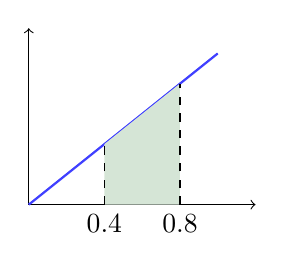
\begin{tikzpicture}[scale=0.8]
            \draw[->] (0,0) -- (3.6,0);
            \draw[->] (0,0) -- (0,2.8);
            \draw[thick, blue!75] (0,0) -- (3,2.4);
            \fill[probExampleGreen!20] (1.2,0) -- (1.2,0.96) -- (2.4,1.92) -- (2.4,0) -- cycle;
            \draw[dashed] (1.2,0) node[below] {0.4} -- (1.2,0.96);
            \draw[dashed] (2.4,0) node[below] {0.8} -- (2.4,1.92);
        \end{tikzpicture}
    }
\end{questionworkspace}
\end{frame}

\begin{frame}[shrink=8]{Soru 26: Lazer Sensörü Hata Bandı Çözümü}
\small
\begin{solutionblock}{Adım 1: Aralık olasılığını integral ile hesapla}
    Sürekli değişkende olasılık alanla hesaplanır:
    \[
    P(0.4 \le X \le 0.8)=\int_{0.4}^{0.8} 2x\,dx
    \]
    \[
    =[x^2]_{0.4}^{0.8}=0.64-0.16=0.48
    \]
\end{solutionblock}

\begin{solutionblock}{Adım 2: Tek nokta olasılığını yorumla}
    Tek bir noktanın altında alan olmadığı için
    \[
    P(X=0.6)=0
    \]
    olur.
\end{solutionblock}

\begin{resultblock}{Yorum}
    Sürekli modellerde ``tam olarak 0.6'' değil, ``0.6 civarında bir bant'' anlamlıdır. Bu ayrım, PDF ile PMF arasındaki en kritik farklardan biridir.
\end{resultblock}
\end{frame}

\subsection{PDF Kavramının Rolü}

\begin{frame}{Yoğunluk Fonksiyonu Perspektifi}
\small
\begin{columns}[T,onlytextwidth]
    \begin{column}{0.56\textwidth}
        \begin{block}{PDF Neyi Gösterir?}
            Yoğunluk fonksiyonu $f(x)$, olasılığın değer ekseni üzerinde \textbf{nasıl yoğunlaştığını} gösterir.
        \end{block}

        \begin{itemize}
            \item $f(x) \ge 0$
            \item $\int_{-\infty}^{\infty} f(x)\,dx = 1$
            \item $P(a \le X \le b)=\int_a^b f(x)\,dx$
        \end{itemize}

        Yoğunluğun büyük olduğu bölgelerde gözlemler daha sık beklenir.
    \end{column}
    \begin{column}{0.40\textwidth}
        \begin{alertblock}{Dikkat}
            PDF'nin belirli bir noktadaki yüksekliği, tek başına olasılık değildir.

            \vspace{0.15cm}
            Olasılık, \textbf{eğri altındaki alan} ile okunur.
        \end{alertblock}

        \begin{infoblock}{Sezgi}
            Aynı toplam alana sahip iki dağılım, olasılığı farklı bölgelerde yoğunlaştırabilir.
        \end{infoblock}
    \end{column}
\end{columns}
\end{frame}

\begin{frame}[t]{Soru 27: Kaynak Robotu Hizalama Hatası}
\small
\begin{questionworkspace}
    Bir kaynak robotunun hizalama hatası $X$ (mm) için
    \[
    f(x)=k(1-x), \quad 0 \le x \le 1
    \]
    veriliyor.

    \vspace{0.15cm}
    \begin{itemize}
        \item Sabit $k$ kaçtır?
        \item Hatanın 0.25 mm'den küçük olma olasılığı nedir?
    \end{itemize}
    \setquestionvisual{
        \centering
        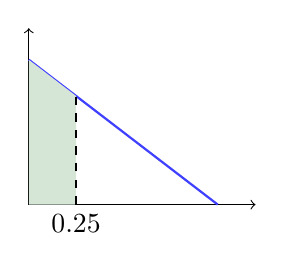
\begin{tikzpicture}[scale=0.8]
            \draw[->] (0,0) -- (3.6,0);
            \draw[->] (0,0) -- (0,2.8);
            \draw[thick, blue!75] (0,2.3) -- (3,0);
            \fill[probExampleGreen!20] (0,0) -- (0,2.3) -- (0.75,1.725) -- (0.75,0) -- cycle;
            \draw[dashed] (0.75,0) node[below] {0.25} -- (0.75,1.725);
        \end{tikzpicture}
    }
\end{questionworkspace}
\end{frame}

\begin{frame}{Soru 27: Kaynak Robotu Hizalama Hatası Çözümü I}
\small
\begin{solutionblock}{Adım 1: Yoğunluğu normalize et}
    PDF'nin toplam alanı 1 olmalıdır:
    \[
    \int_0^1 k(1-x)\,dx
    =k\left[x-\frac{x^2}{2}\right]_0^1
    =\frac{k}{2}=1
    \]
    Buradan
    \[
    k=2
    \]
    bulunur.
\end{solutionblock}
\begin{infoblock}{Geçiş Notu}
    Model geçerli hale geldiğine göre artık sabiti yerine koyup istenen aralık altında kalan alanı hesaplayabiliriz.
\end{infoblock}
\end{frame}

\begin{frame}{Soru 27: Kaynak Robotu Hizalama Hatası Çözümü II}
\small
\begin{solutionblock}{Adım 2: İstenen aralık olasılığını hesapla}
    \[
    P(X<0.25)=\int_0^{0.25} 2(1-x)\,dx
    \]
    \[
    =2\left[x-\frac{x^2}{2}\right]_0^{0.25}
    =2\left(0.25-\frac{0.25^2}{2}\right)=0.4375
    \]
\end{solutionblock}

\begin{resultblock}{Yorum}
    Çözümün ilk yarısı modeli geçerli hale getirir, ikinci yarısı olasılığı hesaplar. Sürekli sorularda bu iki adımı birbirine karıştırmamak gerekir.
\end{resultblock}
\end{frame}

\section{Sürekli Düzgün Dağılım}
\subsection{Düzgün Yoğunluk Yapısı}

\begin{frame}{Sabit Yoğunluk Fikri}
\small
\begin{columns}[T,onlytextwidth]
    \begin{column}{0.56\textwidth}
        \begin{block}{Tanım}
            $X \sim U(A,B)$ ise yoğunluk her noktada aynıdır:
            \[
            f(x)=\frac{1}{B-A}, \quad A \le x \le B
            \]
            ve bunun dışında $0$'dır.
        \end{block}

        \begin{itemize}
            \item Tüm alt aralıklar, uzunluklarıyla orantılı olasılık taşır.
            \item Düzgün dağılım, \textbf{``her yer eşit yoğunlukta''} modelidir.
        \end{itemize}
    \end{column}
    \begin{column}{0.40\textwidth}
        \begin{infoblock}{Kısa Yol}
            \[
            P(c \le X \le d)=\frac{d-c}{B-A}
            \]
            Yani \textbf{istenen uzunluk / toplam uzunluk}.
        \end{infoblock}

        \begin{infoblock}{Uygun Kullanım}
            Rastgele başlangıç zamanı, faz açısı veya bir bant içinde eşit dağılan konumlar.
        \end{infoblock}
    \end{column}
\end{columns}
\end{frame}

\begin{frame}[t]{Soru 28: Robot Kolunun Açısal Sapması}
\small
\begin{questionworkspace}
    Bir robot kolu kalibrasyon sonrasında $-2^\circ$ ile $2^\circ$ arasında eşit olasılıkla konumlanıyor.

    \vspace{0.15cm}
    $X \sim U(-2,2)$ iken kolun
    \[
    -0.5^\circ \le X \le 0.5^\circ
    \]
    aralığında kalma olasılığı nedir?
    \setquestionvisual{
        \centering
        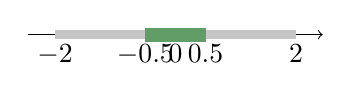
\begin{tikzpicture}[scale=0.85]
            \draw[->] (0,0) -- (4.4,0);
            \draw[line width=3pt, gray!45] (0.4,0) -- (4.0,0);
            \draw[line width=5pt, probExampleGreen!75] (1.75,0) -- (2.65,0);
            \node[below] at (0.4,0) {$-2$};
            \node[below] at (1.75,0) {$-0.5$};
            \node[below] at (2.2,0) {$0$};
            \node[below] at (2.65,0) {$0.5$};
            \node[below] at (4.0,0) {$2$};
        \end{tikzpicture}
    }
\end{questionworkspace}
\end{frame}

\begin{frame}[shrink=8]{Soru 28: Robot Kolunun Açısal Sapması Çözümü}
\small
\begin{solutionblock}{Adım 1: Toplam bant genişliğini bul}
    Düzgün dağılımda olasılık uzunluk oranı ile hesaplanır. Toplam aralık uzunluğu
    \[
    B-A=2-(-2)=4
    \]
    derecedir.
\end{solutionblock}

\begin{solutionblock}{Adım 2: İstenen aralığın uzunluğunu hesapla}
    \[
    0.5-(-0.5)=1
    \]
    derece olduğundan
    \[
    P(-0.5 \le X \le 0.5)=\frac{1}{4}=0.25
    \]
    bulunur.
\end{solutionblock}

\begin{resultblock}{Yorum}
    Düzgün modelde belirleyici olan tek şey aralık uzunluğudur. İstenen tolerans bandı toplam bandın dörtte biri olduğu için olasılık da dörtte birdir.
\end{resultblock}
\end{frame}

\subsection{Düzgün Dağılımın Özellikleri}

\begin{frame}{Ortalama ve Varyansın Yapısı}
\small
\begin{columns}[T,onlytextwidth]
    \begin{column}{0.56\textwidth}
        \begin{block}{Temel Sonuçlar}
            $X \sim U(A,B)$ için:
            \[
            E(X)=\frac{A+B}{2},
            \qquad
            Var(X)=\frac{(B-A)^2}{12}
            \]
        \end{block}

        \begin{itemize}
            \item Ortalama, aralığın tam ortasıdır.
            \item Varyans, bandın genişliği arttıkça büyür.
        \end{itemize}
    \end{column}
    \begin{column}{0.40\textwidth}
        \begin{infoblock}{Sezgi}
            Simetrik bir dağılım olduğu için denge noktası orta noktadadır.

            \vspace{0.15cm}
            Aralık iki katına çıkarsa varyans dört katına çıkar.
        \end{infoblock}
    \end{column}
\end{columns}
\end{frame}

\begin{frame}[t]{Soru 29: CNC Kesim Süresi}
\small
\begin{questionworkspace}
    Bir CNC makinesinde tek bir parçanın kesim süresi 8 ile 14 dakika arasında düzgün dağılım gösteriyor:
    \[
    X \sim U(8,14)
    \]

    \vspace{0.15cm}
    Ortalama süre, varyans ve standart sapma nedir?
    \setquestionvisual{
        \centering
        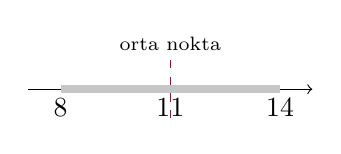
\begin{tikzpicture}[scale=0.82]
            \draw[->] (0,0) -- (4.4,0);
            \draw[line width=3pt, gray!45] (0.5,0) -- (3.9,0);
            \draw[dashed, probSolutionBurgundy] (2.2,-0.45) -- (2.2,0.45);
            \node[below] at (0.5,0) {8};
            \node[below] at (2.2,0) {11};
            \node[below] at (3.9,0) {14};
            \node[above, font=\scriptsize] at (2.2,0.45) {orta nokta};
        \end{tikzpicture}
    }
\end{questionworkspace}
\end{frame}

\begin{frame}[shrink=8]{Soru 29: CNC Kesim Süresi Çözümü}
\small
\begin{solutionblock}{Adım 1: Düzgün dağılımın hazır formüllerini kullan}
    \[
    E(X)=\frac{A+B}{2}, \qquad Var(X)=\frac{(B-A)^2}{12}
    \]
    burada $A=8$ ve $B=14$'tür.
\end{solutionblock}

\begin{solutionblock}{Adım 2: Sayısal değerleri hesapla}
    \[
    E(X)=\frac{8+14}{2}=11 \text{ dk}
    \]
    \[
    Var(X)=\frac{(14-8)^2}{12}=\frac{36}{12}=3
    \]
    \[
    \sigma=\sqrt{3}\approx 1.73 \text{ dk}
    \]
\end{solutionblock}

\begin{resultblock}{Yorum}
    Ortalama 11 dakika olsa da gerçek üretim süreleri 8 ile 14 arasında yayılır. Standart sapma bu yayılımın büyüklüğünü dakika cinsinden ifade eder.
\end{resultblock}
\end{frame}

\section{Üstel Dağılım}
\subsection{Bekleme Süresi Modelleri}

\begin{frame}{Sürekli Zaman ve Olay Bekleme}
\small
\begin{columns}[T,onlytextwidth]
    \begin{column}{0.56\textwidth}
        \begin{block}{Temel Model}
            Bir olayın oluşmasını bekleme süresi üstel dağılımla modellenebilir:
            \[
            X \sim Exp(\lambda), \qquad f(x)=\lambda e^{-\lambda x}, \; x \ge 0
            \]
        \end{block}

        \begin{itemize}
            \item $x<0$ için olasılık yoktur.
            \item $\lambda$ artarsa bekleme süresi kısalır.
            \item Arıza, paket gelişi, müşteri gelişi gibi olaylarda kullanılır.
        \end{itemize}
    \end{column}
    \begin{column}{0.40\textwidth}
        \begin{infoblock}{Kümülatif Olasılık}
            \[
            P(X \le t)=1-e^{-\lambda t}
            \]
            ifadesi, olayın $t$ zamanından önce gerçekleşme olasılığını verir.
        \end{infoblock}
    \end{column}
\end{columns}
\end{frame}

\begin{frame}[t]{Soru 30: Sunucuya İlk Yüksek Öncelikli İstek}
\small
\begin{questionworkspace}
    Bir sunucuya ilk yüksek öncelikli isteğin geliş süresi dakika cinsinden üstel dağılıma sahip:
    \[
    X \sim Exp(0.5)
    \]

    \vspace{0.15cm}
    İsteğin ilk 2 dakika içinde gelme olasılığı nedir?
    \setquestionvisual{
        \centering
        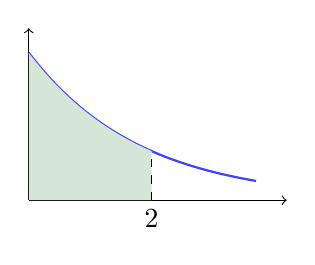
\begin{tikzpicture}[scale=0.78]
            \draw[->] (0,0) -- (4.2,0);
            \draw[->] (0,0) -- (0,2.8);
            \draw[thick, blue!75, domain=0:3.7, smooth, variable=\x] plot ({\x},{2.4*exp(-0.55*\x)});
            \fill[probExampleGreen!20] (0,0) -- plot[domain=0:2, smooth] ({\x},{2.4*exp(-0.55*\x)}) -- (2,0) -- cycle;
            \draw[dashed] (2,0) node[below] {2} -- (2,{2.4*exp(-1.1)});
        \end{tikzpicture}
    }
\end{questionworkspace}
\end{frame}

\begin{frame}[shrink=8]{Soru 30: Sunucuya İlk Yüksek Öncelikli İstek Çözümü}
\small
\begin{solutionblock}{Adım 1: Üstel dağılımın CDF'sini kullan}
    Üstel modelde
    \[
    P(X \le t)=1-e^{-\lambda t}
    \]
    olduğundan burada $t=2$ ve $\lambda=0.5$ alınır.
\end{solutionblock}

\begin{solutionblock}{Adım 2: Sayısal değeri hesapla}
    \[
    P(X \le 2)=1-e^{-0.5\cdot 2}=1-e^{-1}
    \]
    \[
    \approx 1-0.3679=0.6321
    \]
\end{solutionblock}

\begin{resultblock}{Yorum}
    İlk 2 dakika içinde kritik istek gelme olasılığı yaklaşık \%63.2'dir. Üstel model, ``ne kadar süre içinde olay olur?'' sorusuna doğrudan yanıt verir.
\end{resultblock}
\end{frame}

\subsection{Üstel Dağılımın Özellikleri}

\begin{frame}{Hafızasızlık Özelliği}
\small
\begin{columns}[T,onlytextwidth]
    \begin{column}{0.56\textwidth}
        \begin{block}{Hafızasızlık}
            Üstel dağılımın en ayırt edici özelliği
            \[
            P(X>s+t \mid X>s)=P(X>t)
            \]
            biçimindedir.
        \end{block}

        \begin{itemize}
            \item Geçen bekleme süresi, gelecekteki beklemeyi etkilemez.
            \item Sistem yaşlanmıyormuş gibi davranır.
        \end{itemize}
    \end{column}
    \begin{column}{0.40\textwidth}
        \begin{infoblock}{Model Yorumu}
            Poisson süreçlerinden gelen bekleme sürelerinde bu özellik doğaldır.

            \vspace{0.15cm}
            Güçlü aşınma etkileri varsa her zaman gerçekçi olmayabilir.
        \end{infoblock}
    \end{column}
\end{columns}
\end{frame}

\begin{frame}[t]{Soru 31: Alarm Gelmediğinde Kalan Bekleme}
\small
\begin{questionworkspace}
    Bir izleme sisteminde kritik alarm gelene kadar geçen süre saat cinsinden
    \[
    X \sim Exp(0.25)
    \]
    olsun.

    \vspace{0.15cm}
    3 saat boyunca alarm gelmediği biliniyorsa, en az 2 saat daha alarm gelmeme olasılığı nedir?
    \setquestionvisual{
        \centering
        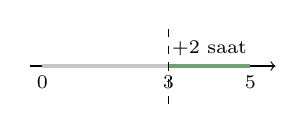
\begin{tikzpicture}[scale=0.8, every node/.style={font=\scriptsize}]
            \draw[->] (0.2,1.4) -- (4.1,1.4);
            \draw[very thick, gray!45] (0.4,1.4) -- (2.4,1.4);
            \draw[very thick, probExampleGreen!70] (2.4,1.4) -- (3.7,1.4);
            \draw[dashed] (2.4,0.8) -- (2.4,2.0);
            \node[below] at (0.4,1.4) {0};
            \node[below] at (2.4,1.4) {3};
            \node[below] at (3.7,1.4) {5};
            \node[above] at (3.05,1.4) {+2 saat};
        \end{tikzpicture}
    }
\end{questionworkspace}
\end{frame}

\begin{frame}{Soru 31: Alarm Gelmediğinde Kalan Bekleme Çözümü I}
\small
\begin{solutionblock}{Adım 1: Hafızasızlık özelliğini uygula}
    Sorulan olasılık
    \[
    P(X>5 \mid X>3)
    \]
    biçimindedir. Üstel dağılım hafızasız olduğu için
    \[
    P(X>5 \mid X>3)=P(X>2)
    \]
    olur.
\end{solutionblock}
\begin{infoblock}{Geçiş Notu}
    Şartlı ifade sadeleşti. Bundan sonra klasik sağ kuyruk formülünü doğrudan uygulayabiliriz.
\end{infoblock}
\end{frame}

\begin{frame}{Soru 31: Alarm Gelmediğinde Kalan Bekleme Çözümü II}
\small
\begin{solutionblock}{Adım 2: Sağ kuyruk olasılığını hesapla}
    Üstel dağılımda
    \[
    P(X>t)=e^{-\lambda t}
    \]
    olduğundan
    \[
    P(X>2)=e^{-0.25\cdot 2}=e^{-0.5}\approx 0.6065
    \]
    bulunur.
\end{solutionblock}

\begin{resultblock}{Yorum}
    Geçen 3 saat, kalan bekleme olasılığını değiştirmez. Bu, üstel dağılımı diğer birçok bekleme modeli karşısında özel yapan özelliktir.
\end{resultblock}
\end{frame}

\section{Normal (Gauss) Dağılım}
\subsection{Normal Dağılımın Motivasyonu}

\begin{frame}{Doğal ve Ölçümsel Süreçler}
\small
\begin{columns}[T,onlytextwidth]
    \begin{column}{0.56\textwidth}
        \begin{block}{Neden Normal?}
            Birçok ölçümsel değişken, çok sayıdaki küçük ve bağımsız etkinin toplamından doğar.
        \end{block}

        \begin{itemize}
            \item Sıcaklık dalgalanması
            \item Takım aşınması
            \item Titreşim
            \item Operatör farkı
        \end{itemize}

        Bu nedenle çap, uzunluk, voltaj, gürültü gibi nicelikler sıklıkla normal modele yakın olur.
    \end{column}
    \begin{column}{0.40\textwidth}
        \begin{infoblock}{Görsel Sezgi}
            Orta değerler daha sık, uç değerler daha seyrektir.

            \vspace{0.15cm}
            Bu davranış çan eğrisi ile temsil edilir.
        \end{infoblock}
    \end{column}
\end{columns}
\end{frame}

\begin{frame}[t]{Soru 32: Baskı Devre Delik Çapı}
\small
\begin{questionworkspace}
    Bir baskı devre kartındaki delik çapını; matkap titreşimi, sıcaklık, malzeme sertliği ve operatör ayarı gibi çok sayıda küçük etki birlikte belirliyor.

    \vspace{0.15cm}
    Bu ölçüm için hangi dağılım daha uygun ilk model olur ve neden?
    \setquestionvisual{
        \centering
        \begin{tikzpicture}[scale=0.85, every node/.style={font=\scriptsize}]
            \node[qbox] (m) at (2.1,1.4) {Delik çapı};
            \node[qgreen] (a) at (0.3,2.6) {Titreşim};
            \node[qgreen] (b) at (3.9,2.6) {Sıcaklık};
            \node[qgreen] (c) at (0.3,0.2) {Malzeme};
            \node[qgreen] (d) at (3.9,0.2) {Operatör};
            \draw[qline] (a) -- (m);
            \draw[qline] (b) -- (m);
            \draw[qline] (c) -- (m);
            \draw[qline] (d) -- (m);
        \end{tikzpicture}
    }
\end{questionworkspace}
\end{frame}

\begin{frame}[shrink=8]{Soru 32: Baskı Devre Delik Çapı Çözümü}
\small
\begin{solutionblock}{Adım 1: Sürecin yapısını yorumla}
    Burada tek bir baskın neden yoktur; sonuç, çok sayıda küçük etkinin toplam davranışıyla oluşur.
\end{solutionblock}

\begin{solutionblock}{Adım 2: Uygun modeli seç}
    Bu tür ölçümlerde ilk doğal model \textbf{normal dağılım}dır. Çünkü
    \begin{itemize}
        \item merkezi değerlerin çevresinde yığılma beklenir,
        \item aşırı küçük ve aşırı büyük değerler daha seyrek görülür,
        \item çok sayıda küçük etki toplamı çan eğrisi davranışına yaklaşır.
    \end{itemize}
\end{solutionblock}

\begin{resultblock}{Yorum}
    Gerçek veri her zaman tam normal olmayabilir; ancak süreç fiziği böyle bir toplam etki yapısı gösteriyorsa normal dağılım iyi bir başlangıç modelidir.
\end{resultblock}
\end{frame}

\subsection{Normal Yoğunluk Fonksiyonu}

\begin{frame}{Parametreler ($\mu$, $\sigma$)}
\small
\begin{columns}[T,onlytextwidth]
    \begin{column}{0.56\textwidth}
        \begin{block}{Yoğunluk}
            \[
            f(x)=\frac{1}{\sigma\sqrt{2\pi}}
            \exp\!\left(-\frac{(x-\mu)^2}{2\sigma^2}\right)
            \]
        \end{block}

        \begin{itemize}
            \item $\mu$: merkezin konumu
            \item $\sigma$: yayılımın genişliği
        \end{itemize}
    \end{column}
    \begin{column}{0.40\textwidth}
        \begin{infoblock}{Yorum}
            $\mu$ değişirse eğri sola-sağa kayar.

            \vspace{0.15cm}
            $\sigma$ büyürse eğri yayvanlaşır; küçülürse daralır.
        \end{infoblock}
    \end{column}
\end{columns}
\end{frame}

\begin{frame}[t]{Soru 33: Dolum Ağırlığının Konumu}
\small
\begin{questionworkspace}
    Bir dolum hattında paket ağırlıkları
    \[
    X \sim N(500,\;4^2)
    \]
    ile modelleniyor.

    \vspace{0.15cm}
    508 gram ölçümü ortalamadan kaç standart sapma uzaktadır ve ortalamanın hangi tarafındadır?
    \setquestionvisual{
        \centering
        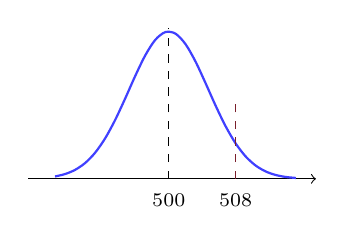
\begin{tikzpicture}[scale=0.85]
            \draw[->] (0,0) -- (4.3,0);
            \draw[thick, blue!75, domain=0.4:4.0, smooth, variable=\x] plot ({\x},{2.2*exp(-(\x-2.1)^2/0.7)});
            \draw[dashed] (2.1,0) -- (2.1,2.25);
            \draw[dashed, probSolutionBurgundy] (3.1,0) -- (3.1,1.15);
            \node[below=2pt, font=\scriptsize] at (2.1,0) {500};
            \node[below=2pt, font=\scriptsize] at (3.1,0) {508};
        \end{tikzpicture}
    }
\end{questionworkspace}
\end{frame}

\begin{frame}[shrink=8]{Soru 33: Dolum Ağırlığının Konumu Çözümü}
\small
\begin{solutionblock}{Adım 1: Z-dönüşümünü uygula}
    \[
    z=\frac{x-\mu}{\sigma}=\frac{508-500}{4}=2
    \]
\end{solutionblock}

\begin{solutionblock}{Adım 2: İşaret ve büyüklüğü yorumla}
    $z=2$ pozitif olduğu için 508 gram, ortalamanın sağ tarafındadır. Ayrıca mutlak değer olarak 2 olduğundan gözlem, ortalamanın \textbf{2 standart sapma} üzerindedir.
\end{solutionblock}

\begin{resultblock}{Yorum}
    Z-skoru, doğrudan olasılık vermese de gözlemin ne kadar sıra dışı olduğunu hızlı biçimde anlatır. Aynı mantık, farklı süreçleri karşılaştırmada da kullanılır.
\end{resultblock}
\end{frame}

\subsection{Normal Dağılımın Temel Özellikleri}

\begin{frame}{Simetri, Tepe Noktası ve Yayılım}
\small
\begin{columns}[T,onlytextwidth]
    \begin{column}{0.56\textwidth}
        \begin{block}{Temel Özellikler}
            \begin{itemize}
                \item Dağılım $\mu$ etrafında simetriktir.
                \item Ortalama = medyan = mod = $\mu$
                \item Tepe noktası merkezde bulunur.
            \end{itemize}
        \end{block}

        \begin{block}{Yayılım Kuralı}
            Yaklaşık olarak:
            \[
            P(\mu-\sigma \le X \le \mu+\sigma) \approx 0.68
            \]
        \end{block}
    \end{column}
    \begin{column}{0.40\textwidth}
        \begin{infoblock}{Devamı}
            \[
            P(\mu-2\sigma \le X \le \mu+2\sigma) \approx 0.95
            \]
            \[
            P(\mu-3\sigma \le X \le \mu+3\sigma) \approx 0.997
            \]
        \end{infoblock}
    \end{column}
\end{columns}
\end{frame}

\begin{frame}[t]{Soru 34: Rulman Çapı Toleransı}
\small
\begin{questionworkspace}
    Bir rulman çapı
    \[
    X \sim N(50,\;0.1^2)
    \]
    ile modelleniyor.

    \vspace{0.15cm}
    Parçanın
    \[
    49.9 \le X \le 50.1
    \]
    aralığında kalma olasılığı yaklaşık olarak nedir?
    \setquestionvisual{
        \centering
        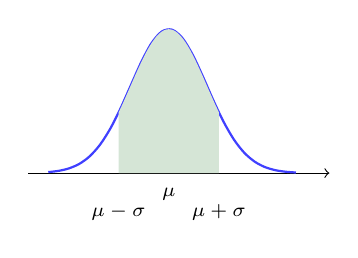
\begin{tikzpicture}[scale=0.85]
            \draw[->] (0,0) -- (4.5,0);
            \draw[thick, blue!75, domain=0.3:4.0, smooth, variable=\x] plot ({\x},{2.15*exp(-(\x-2.1)^2/0.65)});
            \fill[probExampleGreen!20] (1.35,0) -- plot[domain=1.35:2.85, smooth] ({\x},{2.15*exp(-(\x-2.1)^2/0.65)}) -- (2.85,0) -- cycle;
            \node[below=8pt, font=\scriptsize] at (1.35,0) {$\mu-\sigma$};
            \node[below=2pt, font=\scriptsize] at (2.1,0) {$\mu$};
            \node[below=8pt, font=\scriptsize] at (2.85,0) {$\mu+\sigma$};
        \end{tikzpicture}
    }
\end{questionworkspace}
\end{frame}

\begin{frame}[shrink=8]{Soru 34: Rulman Çapı Toleransı Çözümü}
\small
\begin{solutionblock}{Adım 1: Bandın standart sapma cinsinden konumunu belirle}
    Burada ortalama $\mu=50$ ve standart sapma $\sigma=0.1$'dir. Verilen aralık
    \[
    50-0.1 \le X \le 50+0.1
    \]
    yani
    \[
    \mu-\sigma \le X \le \mu+\sigma
    \]
    bandıdır.
\end{solutionblock}

\begin{solutionblock}{Adım 2: 68-95-99.7 kuralını uygula}
    Yaklaşık kurala göre
    \[
    P(\mu-\sigma \le X \le \mu+\sigma)\approx 0.68
    \]
    olur.
\end{solutionblock}

\begin{resultblock}{Yorum}
    Üretimin yaklaşık \%68'i bu dar tolerans bandında kalır. Bu soru, tablo kullanmadan hızlı yaklaşık yorum yapmayı gösterir.
\end{resultblock}
\end{frame}

\section{Standart Normal Dağılım ve Dönüşüm}
\subsection{Standardizasyon Fikri}

\begin{frame}{Z-Dönüşümü}
\small
\begin{columns}[T,onlytextwidth]
    \begin{column}{0.56\textwidth}
        \begin{block}{Dönüşüm}
            Her normal değişken
            \[
            Z=\frac{X-\mu}{\sigma}
            \]
            dönüşümü ile standart normal dağılıma taşınır.
        \end{block}

        \begin{itemize}
            \item Yeni dağılım: $Z \sim N(0,1)$
            \item Farklı birimlerdeki normal soruları tek tabloya indirger.
        \end{itemize}
    \end{column}
    \begin{column}{0.40\textwidth}
        \begin{infoblock}{Yorum}
            $z$ değeri, gözlemin ortalamadan kaç standart sapma uzakta olduğunu söyler.
        \end{infoblock}
    \end{column}
\end{columns}
\end{frame}

\begin{frame}[t]{Soru 35: İki Batarya Testini Karşılaştırma}
\small
\begin{questionworkspace}
    İki ayrı batarya ömrü testi için aşağıdaki ölçümler elde ediliyor:
    \begin{itemize}
        \item Test A: $X_A \sim N(120,15^2)$ ve ölçüm 150 dk
        \item Test B: $X_B \sim N(80,8^2)$ ve ölçüm 92 dk
    \end{itemize}

    Hangi sonuç, kendi sürecine göre daha sıra dışıdır?
    \setquestionvisual{
        \centering
        \renewcommand{\arraystretch}{1.3}
        \setlength{\tabcolsep}{10pt}
        \begin{tabular}{@{}lcc@{}}
            \toprule
            Test & Ölçüm & Ölçek \\ \midrule
            A & 150 & $(120,15)$ \\
            B & 92 & $(80,8)$ \\ \bottomrule
        \end{tabular}

        \vspace{0.15cm}
        {\scriptsize ortak kıyas: z-skoru}
    }
\end{questionworkspace}
\end{frame}

\begin{frame}[shrink=8]{Soru 35: İki Batarya Testini Karşılaştırma Çözümü}
\small
\begin{solutionblock}{Adım 1: İki sonucu aynı ölçeğe taşı}
    Doğrudan dakika cinsinden kıyas yapmak doğru değildir; çünkü süreçlerin yayılımları farklıdır. Bu yüzden her ölçümü z-skoruna çeviririz:
    \[
    z_A=\frac{150-120}{15}=2
    \]
    \[
    z_B=\frac{92-80}{8}=1.5
    \]
\end{solutionblock}

\begin{solutionblock}{Adım 2: Mutlak z-skorlarını karşılaştır}
    \[
    |z_A|=2,\qquad |z_B|=1.5
    \]
    olduğundan Test A'daki 150 dakikalık sonuç, kendi sürecine göre daha sıra dışıdır.
\end{solutionblock}

\begin{resultblock}{Yorum}
    Standardizasyon, farklı ölçeklerdeki ölçümleri ortak zemine taşır. Ham değer büyük görünse bile asıl sıra dışılık, standart sapma cinsinden uzaklıkla anlaşılır.
\end{resultblock}
\end{frame}

\subsection{Z-Tablosu ile Olasılık Hesabı}

\begin{frame}{Sol Taraf Alanları}
\small
\begin{columns}[T,onlytextwidth]
    \begin{column}{0.56\textwidth}
        \begin{block}{Tablo Ne Verir?}
            Standart normal tabloları genellikle
            \[
            \Phi(z)=P(Z \le z)
            \]
            değerini verir.
        \end{block}

        \begin{itemize}
            \item Önce $X$ değerini $z$'ye çeviririz.
            \item Sonra tablodan soldaki alanı okuruz.
        \end{itemize}
    \end{column}
    \begin{column}{0.40\textwidth}
        \begin{infoblock}{Kuyruk Dönüşümü}
            \[
            P(Z>z)=1-\Phi(z)
            \]
            \[
            P(a<Z<b)=\Phi(b)-\Phi(a)
            \]
        \end{infoblock}
    \end{column}
\end{columns}
\end{frame}

\begin{frame}[t]{Soru 36: Kaplama Kalınlığı Aralığı}
\small
\begin{questionworkspace}
    Bir kaplama kalınlığı
    \[
    X \sim N(40,3^2)
    \]
    ile modelleniyor.

    \vspace{0.15cm}
    \[
    P(38 \le X \le 44)
    \]
    olasılığını bulunuz.
    \setquestionvisual{
        \centering
        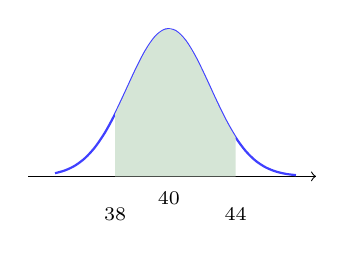
\begin{tikzpicture}[scale=0.85]
            \draw[->] (0,0) -- (4.3,0);
            \draw[thick, blue!75, domain=0.4:4.0, smooth, variable=\x] plot ({\x},{2.2*exp(-(\x-2.1)^2/0.75)});
            \fill[probExampleGreen!20] (1.3,0) -- plot[domain=1.3:3.1, smooth] ({\x},{2.2*exp(-(\x-2.1)^2/0.75)}) -- (3.1,0) -- cycle;
            \node[below=8pt, font=\scriptsize] at (1.3,0) {38};
            \node[below=2pt, font=\scriptsize] at (2.1,0) {40};
            \node[below=8pt, font=\scriptsize] at (3.1,0) {44};
        \end{tikzpicture}
    }
\end{questionworkspace}
\end{frame}

\begin{frame}[shrink=8]{Soru 36: Kaplama Kalınlığı Aralığı Çözümü}
\small
\begin{solutionblock}{Adım 1: Alt ve üst sınırı standartlaştır}
    \[
    z_1=\frac{38-40}{3}=-0.67,\qquad
    z_2=\frac{44-40}{3}=1.33
    \]
\end{solutionblock}

\begin{solutionblock}{Adım 2: Tablodan alanları okuyup fark al}
    \[
    \Phi(1.33)\approx 0.9082,\qquad \Phi(-0.67)\approx 0.2514
    \]
    \[
    P(38 \le X \le 44)=\Phi(1.33)-\Phi(-0.67)
    =0.9082-0.2514=0.6568
    \]
\end{solutionblock}

\begin{resultblock}{Yorum}
    Z-tablosu sorularında ana akış hep aynıdır: sınırları standartlaştır, soldaki alanları oku, gerekiyorsa fark veya tümleyen al.
\end{resultblock}
\end{frame}

\begin{frame}[t]{Soru 37: Yüzde 90 Sınırını Bulma}
\small
\begin{questionworkspace}
    Bir motor milinin ölçümü
    \[
    X \sim N(25,\;0.4^2)
    \]
    olsun.

    \vspace{0.15cm}
    Ölçümlerin \%90'ının altında kaldığı üst sınır $x_{0.90}$ nedir?
    \setquestionvisual{
        \centering
        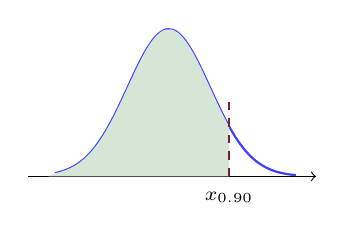
\begin{tikzpicture}[scale=0.85]
            \draw[->] (0,0) -- (4.3,0);
            \draw[thick, blue!75, domain=0.4:4.0, smooth, variable=\x] plot ({\x},{2.2*exp(-(\x-2.1)^2/0.75)});
            \fill[probExampleGreen!20] (0.3,0) -- plot[domain=0.4:3.0, smooth] ({\x},{2.2*exp(-(\x-2.1)^2/0.75)}) -- (3.0,0) -- cycle;
            \draw[dashed, probSolutionBurgundy] (3.0,0) -- (3.0,1.2);
            \node[below=2pt, font=\scriptsize] at (3.0,0) {$x_{0.90}$};
        \end{tikzpicture}
    }
\end{questionworkspace}
\end{frame}

\begin{frame}[shrink=8]{Soru 37: Yüzde 90 Sınırını Bulma Çözümü}
\small
\begin{solutionblock}{Adım 1: Standart normal yüzde 90 noktasını bul}
    \[
    P(Z\le z_{0.90})=0.90
    \]
    için tablodan yaklaşık
    \[
    z_{0.90}\approx 1.28
    \]
    alınır.
\end{solutionblock}

\begin{solutionblock}{Adım 2: Orijinal birime geri dön}
    \[
    x=\mu+z\sigma=25+1.28(0.4)
    \]
    \[
    x=25.512
    \]
\end{solutionblock}

\begin{resultblock}{Yorum}
    Bu değer, sürecin \%90 üst alt sınırlarından biri gibi yorumlanabilir. Yüzdelik sorularında mantık, önce standart yüzde noktasını bulup sonra geri ölçeklemektir.
\end{resultblock}
\end{frame}

\section{Normal Dağılımın Uygulamaları}
\subsection{Ölçüm ve Üretim Süreçleri}

\begin{frame}{Spesifikasyon Aralıkları}
\small
\begin{columns}[T,onlytextwidth]
    \begin{column}{0.56\textwidth}
        \begin{block}{Temel Amaç}
            Üretimde temel soru, bir ölçümün kabul edilen spesifikasyon bandı içinde kalma olasılığıdır.
        \end{block}

        \begin{itemize}
            \item Alt limit: LSL
            \item Üst limit: USL
            \item Hedef: $P(LSL \le X \le USL)$
        \end{itemize}
    \end{column}
    \begin{column}{0.40\textwidth}
        \begin{infoblock}{Yorum}
            Normal model, hurda oranını ve proses yeterliliğini yorumlamada ilk yaklaşımdır.
        \end{infoblock}
    \end{column}
\end{columns}
\end{frame}

\begin{frame}[t]{Soru 38: Mil Çapı Kabul Olasılığı}
\small
\begin{questionworkspace}
    Bir mil çapı
    \[
    X \sim N(12.00,\;0.03^2)
    \]
    ile modelleniyor.

    \vspace{0.15cm}
    Kabul aralığı
    \[
    11.95 \le X \le 12.05
    \]
    olarak veriliyor. Buna göre kabul olasılığı nedir?
    \setquestionvisual{
        \centering
        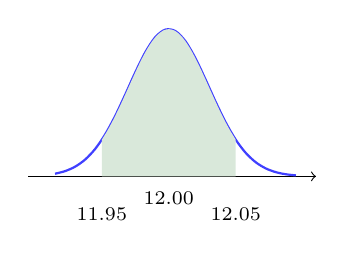
\begin{tikzpicture}[scale=0.85]
            \draw[->] (0,0) -- (4.3,0);
            \draw[thick, blue!75, domain=0.4:4.0, smooth, variable=\x] plot ({\x},{2.2*exp(-(\x-2.1)^2/0.72)});
            \fill[probExampleGreen!18] (1.1,0) -- plot[domain=1.1:3.1, smooth] ({\x},{2.2*exp(-(\x-2.1)^2/0.72)}) -- (3.1,0) -- cycle;
            \node[below=8pt, font=\scriptsize] at (1.1,0) {11.95};
            \node[below=2pt, font=\scriptsize] at (2.1,0) {12.00};
            \node[below=8pt, font=\scriptsize] at (3.1,0) {12.05};
        \end{tikzpicture}
    }
\end{questionworkspace}
\end{frame}

\begin{frame}[shrink=8]{Soru 38: Mil Çapı Kabul Olasılığı Çözümü}
\small
\begin{solutionblock}{Adım 1: Alt ve üst limitleri z-skoruna çevir}
    \[
    z_1=\frac{11.95-12.00}{0.03}=-1.67,\qquad
    z_2=\frac{12.05-12.00}{0.03}=1.67
    \]
\end{solutionblock}

\begin{solutionblock}{Adım 2: Tablo ile kabul alanını hesapla}
    \[
    P(11.95 \le X \le 12.05)=\Phi(1.67)-\Phi(-1.67)
    \]
    \[
    =0.9525-0.0475=0.9050
    \]
\end{solutionblock}

\begin{resultblock}{Yorum}
    Yaklaşık kabul oranı \%90.5'tir. Bu tür sorular, normal dağılımın üretim toleranslarını nicel olarak yorumlamadaki temel kullanım alanıdır.
\end{resultblock}
\end{frame}

\subsection{Yaklaşım Fikirleri}

\begin{frame}{Ayrık Dağılımlara Sürekli Yaklaşım}
\small
\begin{columns}[T,onlytextwidth]
    \begin{column}{0.56\textwidth}
        \begin{block}{Ne Zaman?}
            Ayrık bir değişkenin dağılımı yeterince yumuşaklaştığında normal dağılım yaklaşımı kullanılabilir.
        \end{block}

        \begin{itemize}
            \item Özellikle binom dağılımda $np$ ve $n(1-p)$ yeterince büyükse
            \item Süreklilik düzeltmesi yaklaşımı iyileştirir
        \end{itemize}
    \end{column}
    \begin{column}{0.40\textwidth}
        \begin{resultblock}{Pratik Kazanç}
            Zor toplamalı ayrık hesapları daha hızlı sürekli bir modele taşımak.
        \end{resultblock}
    \end{column}
\end{columns}
\end{frame}

\begin{frame}[t]{Soru 39: Kusurlu Parça Sayısına Normal Yaklaşım}
\small
\begin{questionworkspace}
    Bir hatta 200 parça üretiliyor. Her bir parçanın kusurlu olma olasılığı $p=0.04$.

    \vspace{0.15cm}
    Kusurlu parça sayısı $X \sim Bin(200,0.04)$ iken,
    \[
    P(6 \le X \le 10)
    \]
    olasılığını normal yaklaşımla tahmin ediniz.
    \setquestionvisual{
        \centering
        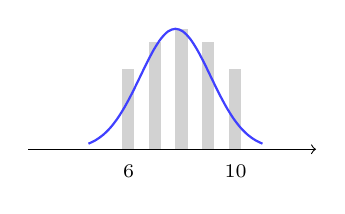
\begin{tikzpicture}[scale=0.85]
            \draw[->] (0,0) -- (4.3,0);
            \foreach \x/\h in {1.4/1.2,1.8/1.6,2.2/1.8,2.6/1.6,3.0/1.2}{
                \fill[gray!35] (\x,0) rectangle ++(0.18,\h);
            }
            \draw[thick, blue!75, domain=0.9:3.5, smooth, variable=\x] plot ({\x},{1.8*exp(-(\x-2.2)^2/0.55)});
            \node[below=2pt, font=\scriptsize] at (1.5,0) {6};
            \node[below=2pt, font=\scriptsize] at (3.1,0) {10};
        \end{tikzpicture}
    }
\end{questionworkspace}
\end{frame}

\begin{frame}[shrink=8]{Soru 39: Kusurlu Parça Sayısına Normal Yaklaşım Çözümü}
\small
\begin{solutionblock}{Adım 1: Binom dağılımın normal yaklaşım parametrelerini kur}
    \[
    \mu=np=200(0.04)=8
    \]
    \[
    \sigma=\sqrt{np(1-p)}=\sqrt{200(0.04)(0.96)}=\sqrt{7.68}\approx 2.77
    \]
\end{solutionblock}

\begin{solutionblock}{Adım 2: Süreklilik düzeltmesi uygula ve standartlaştır}
    \[
    P(6 \le X \le 10)\approx P(5.5 \le Y \le 10.5), \qquad Y\sim N(8,2.77^2)
    \]
    \[
    z_1=\frac{5.5-8}{2.77}\approx -0.90,\qquad
    z_2=\frac{10.5-8}{2.77}\approx 0.90
    \]
    \[
    P\approx \Phi(0.90)-\Phi(-0.90)=0.8159-0.1841=0.6318
    \]
\end{solutionblock}

\begin{resultblock}{Yorum}
    Normal yaklaşım sonucu yaklaşık 0.632'dir. Ayrık bir soruyu sürekli modele taşırken süreklilik düzeltmesi yapılması, yaklaşımı belirgin biçimde iyileştirir.
\end{resultblock}
\end{frame}

\section{Haftanın Kavramsal Özeti}
\subsection{Sürekli Dağılımların Genel Haritası}

\begin{frame}{Düzgün, Üstel, Normal Karşılaştırması}
\small
\centering
\renewcommand{\arraystretch}{1.3}
\begin{tabular}{@{}llll@{}}
    \toprule
    \textbf{Dağılım} & \textbf{Temel Durum} & \textbf{Parametre} & \textbf{Tipik Soru} \\ \midrule
    Düzgün & Her nokta eşit yoğunlukta & $A,B$ & Bant içinde kalma \\
    Üstel & Bir sonraki olayı bekleme & $\lambda$ & Ne kadar beklerim? \\
    Normal & Ölçüm ve toplam etki & $\mu,\sigma$ & Tolerans içinde mi? \\ \bottomrule
\end{tabular}

\vspace{0.25cm}
\begin{columns}[T,onlytextwidth]
    \begin{column}{0.48\textwidth}
        \begin{block}{Düzgün}
            Aralık uzunluğu olasılığı belirler.
        \end{block}
    \end{column}
    \begin{column}{0.48\textwidth}
        \begin{block}{Üstel ve Normal}
            Biri bekleme süresini, diğeri ölçüm yayılımını açıklar.
        \end{block}
    \end{column}
\end{columns}
\end{frame}

\begin{frame}[t]{Soru 40: Hangi Problemde Hangi Dağılım?}
\small
\begin{questionworkspace}
    Aşağıdaki durumları uygun dağılımla eşleştirin:
    \begin{enumerate}
        \item Bir teknisyenin vardiya içinde rastgele başlama anı
        \item Sunucuya bir sonraki acil isteğin geliş süresi
        \item Üretilen bir milin çap ölçümü
    \end{enumerate}
    \setquestionvisual{
        \centering
        \renewcommand{\arraystretch}{1.3}
        \setlength{\tabcolsep}{12pt}
        \begin{tabular}{@{}ll@{}}
            \toprule
            Durum & Aday \\ \midrule
            Bant içi konum & Düzgün \\
            Bekleme süresi & Üstel \\
            Ölçüm değişkeni & Normal \\ \bottomrule
        \end{tabular}
    }
\end{questionworkspace}
\end{frame}

\begin{frame}[shrink=8]{Soru 40: Hangi Problemde Hangi Dağılım? Çözümü}
\small
\begin{solutionblock}{Adım 1: Her problemi yapısına göre sınıflandır}
    \begin{enumerate}
        \item \textbf{Düzgün dağılım}: vardiya içindeki başlangıç anı belirli bir bant içinde eşit olasılıkla düşünülebilir.
        \item \textbf{Üstel dağılım}: bir sonraki isteğin geliş süresi bekleme süresi problemidir.
        \item \textbf{Normal dağılım}: mil çapı çok sayıda küçük üretim etkisinin toplam sonucu olan ölçüm değişkenidir.
    \end{enumerate}
\end{solutionblock}

\begin{resultblock}{Kısa Kural}
    \textbf{Bant içindeki konum} $\rightarrow$ düzgün,\qquad
    \textbf{bekleme süresi} $\rightarrow$ üstel,\qquad
    \textbf{ölçüm ve tolerans} $\rightarrow$ normal.
\end{resultblock}
\end{frame}

\subsection{Haftayı Tamamlarken}

\begin{frame}{Çıkış Bileti: Bu Haftadan Ne Kalmış Olmalı?}
\small
\begin{columns}[T,onlytextwidth]
    \begin{column}{0.48\textwidth}
        \begin{resultblock}{Kavramsal Kontrol}
            \begin{itemize}
                \item Sürekli değişkende neden $P(X=x)=0$?
                \item Düzgün, üstel ve normal dağılım hangi problem tiplerinde doğal modeldir?
                \item Z-dönüşümü neden farklı süreçleri karşılaştırmayı kolaylaştırır?
            \end{itemize}
        \end{resultblock}
    \end{column}
    \begin{column}{0.48\textwidth}
        \begin{exampleblock}{Kendi Kendine Deneme}
            Aşağıdaki üç problemi bir daha çözüp kontrol edin:
            \begin{enumerate}
                \item Bir PDF'yi normalize etme
                \item Bir z-skorunu yorumlama
                \item Bir tolerans bandı olasılığını tablo ile bulma
            \end{enumerate}
        \end{exampleblock}
    \end{column}
\end{columns}
\end{frame}

\section{Kaynaklar}
\begin{frame}[allowframebreaks]
  \frametitle{Kaynaklar}
  \nocite{walpole,walpole_ch4,ross2014first}
  \printbibliography{}
\end{frame}

\appendix

\section{Yapay Zeka Asistanı}
\begin{frame}{Yapay Zeka Asistanınız: NotebookLM}
    \small
    \begin{columns}[T]
        \begin{column}{0.48\textwidth}
            \justifying{}
            \textbf{Ders Materyalleri ile Etkileşime Geçin!}

            Bu dersin sunumları, notları ve yardımcı içerikleri Google'ın gelişmiş yapay zeka asistanı \textbf{NotebookLM} sisteminde düzenlenmiştir.

            \vspace{1em}
            \begin{itemize}
                \item \textbf{Anında Soru Cevap:} Konuya dair kısa ve hedefli sorular sorun.
                \item \textbf{Özetleme:} Uzun bir bölümü hızlıca tekrar edin.
                \item \textbf{Sesli Genel Bakış:} Konuyu podcast benzeri bir akışla dinleyin.
            \end{itemize}

            \vspace{1.2em}
            \begin{center}
                {\setbeamercolor{button}{bg=red,fg=black}
                \href{https://notebooklm.google.com/notebook/1daaa713-b9d0-4bb3-bbe6-defbaf4e67d4}{\beamerbutton{\rule[-4ex]{0pt}{11ex}\Large \textbf{NotebookLM'yi Aç}}}}
            \end{center}
        \end{column}

        \begin{column}{0.48\textwidth}
            \centering
            \includegraphics[width=\textwidth,height=0.6\textheight,keepaspectratio]{figures/notebooklm.jpg}
        \end{column}
    \end{columns}
\end{frame}

\begin{frame}[plain,noframenumbering]
    \begin{tikzpicture}[remember picture,overlay]
        \node[anchor=center, at=(current page.center), inner sep=0pt] {
            \includegraphics[width=\paperwidth,height=\paperheight]{logos/background_figure.jpg}
        };
        \node[
            anchor=center,
            at=(current page.center),
            fill=white!92,
            rounded corners,
            inner sep=14pt,
            text width=0.72\paperwidth,
            align=center
        ] {
            \Large \textbf{Hafta 6 Tamamlandı} \\
            \vspace{0.4em}
            \normalsize Bir sonraki tekrarınızda önce model tipini seçin, sonra doğru olasılık aracını kullanın.\\
            \small Düzgün $\rightarrow$ bant, Üstel $\rightarrow$ bekleme, Normal $\rightarrow$ ölçüm ve tolerans
        };
    \end{tikzpicture}
\end{frame}

\end{document}


